\documentclass{article}
\usepackage[utf8]{inputenc}

\title{UWB Indoor Localization}
\author{Ali Safaei}
\date{May 2020}

\usepackage{amssymb}
\usepackage{graphicx}
\usepackage{epsfig} % for postscript graphics files
\usepackage{epstopdf}
\usepackage{url}
\usepackage{float}
\usepackage{multirow}
\usepackage{color}
\usepackage{amsmath}
%\usepackage{subcaption}
\usepackage{subfig}
\usepackage{minted}
%\usepackage{hyperref}
\begin{document}

\maketitle

\section{Introduction}
Ultra WideBand (UWB) signals are sorted among the RF signals. The special feature of the UWB signal is its crisp pulse (compared to the narrowband signals), which makes it more clear to determine the exact time for its transmission and reception (Figure \ref{Fig_01}).

\begin{figure}[thpb]
\centering
\includegraphics[scale=0.45]{Pics/UWB_signal.PNG}
\caption{Comparison of the amplitudes of the narrowband and ultra-wideband RF signals.}
\label{Fig_01}
\end{figure}

This is an important feature for ranging process based on the time of flight of a signal. More specifically, one can estimate the range (or distance $d$) between the transmitter and the receiver antennas just by accurate measurement of time of flight ($t_f$) for the transmitted signal and then multiplying it with the speed of light ($c$), i.e.
\begin{equation} \label{Eq_01_01}
d = c t_f \;.
\end{equation}
As it is mentioned above, the UWB signals are good for ranging applications as one can measure the time of flight for the corresponding RF signal more accurate compared to the case of WiFi, ZigBee or etc.
The process of determining the distance between two antennas is named as Two-Way Ranging (TWR).
According to the literature of localization, the TWR process can be implemented on two different schemes; Single-sided TWR (i.e. SS-TWR) and Double-sided TWR (i.e. DS-TWR).
A brief introduction of the two schemes are provided here and more elaborated information can be found in the DWM1000 manual document. 

\subsection{Single-Sided Two-way Ranging}
In SS-TWR algorithm, two messages are transmitted between the two devices; the poll message from device-A to device-B and the reply message from device-B to device-A (Figure \ref{Fig_02}).
The propagation time of the signal or the time of flight in an SS-TWR algorithm is computed as follows
\begin{equation} \label{Eq_01_02}
t_f = \frac{t_{round} - t_{reply}}{2} \;,
\end{equation}
where $t_{round}$ is the round-trip time for sending the poll message and receiving the reply message at device-A, while $t_{reply}$ is the time taken in device-B to send the reply message in response to the poll message.

\begin{figure}[thpb]
\centering
\includegraphics[scale=0.6]{Pics/SS_TWR.PNG}
\caption{Schematic for the SS-TWR algorithm.}
\label{Fig_02}
\end{figure}

\subsection{Double-Sided Two-way Ranging}
In DW-TWR algorithm, three messages are transmitted between the two devices; the poll message, the reply message and the final message from device-A to device-B which is sent after receiving the reply message (Fig. \ref{Fig_05}).
The time of flight in an DS-TWR algorithm is computed as follows
\begin{equation} \label{Eq_01_03}
t_f = \frac{t_{round1} \times t_{round2} - t_{reply1} \times t_{reply2}}{t_{round1} + t_{round2} + t_{reply1} + t_{reply2}} \;,
\end{equation}
where the different time periods are depicted in Figure \ref{Fig_03}.

\begin{figure}[thpb]
\centering
\includegraphics[scale=0.65]{Pics/DS_TWR.PNG}
\caption{Schematic for the DS-TWR algorithm.}
\label{Fig_03}
\end{figure}

\newpage
\section{Hardware}

\subsection{DWM1001-Dev module}
DWM1001-dev module is a product of the DecaWave company. The company is located in Ireland. The DWM1001-dev module as depicted in Figure \ref{Fig_04} is actually a developing board containing the DWM1001 module and also a set of pins compatible with the Raspberry Pi 2 and 3 boards. 

\begin{figure}[thpb]
\centering
\includegraphics[scale=0.4]{Pics/DWM1001DEV01.PNG}
\caption{DWM1001-dev module.}
\label{Fig_04}
\end{figure}

Moreover, the DWM1001 module includes the DWM1000 UWB antenna and the nordic nRF52832 microprocessor (Figure \ref{Fig_05}), which is ready to be programmed using codes in C language. SEGGER Embedded Studio is the suggested IDE by DecaWave for preparing and compiling the C codes to be implemented on this microprocessor. 
As can be seen in Figure \ref{Fig_05}, the microprocessor in DWM1001 module has the following communicating protocols:
\begin{itemize}
    \item SPI-1; the first SPI protocol is dedicated to the data transmission between the nRF52832 microprocessor and the DWM1000 antenna. The messages received by the antenna can be sent to the microprocessor via this protocl.
    \item SPI-2; the second SPI protocol is available for the user to communicate with the microprocessor. The command from an outside interface (e.g. the Raspberry Pi computers) can be sent via this protocol. Moreover, the messages transmitted via the UWB antennas can be sent/received using this protocol. 
    \item UART; the UART protocol is the another means that a user can send command to the module and receive the messages from the module. 
    \item I2C; this protocol is already used for receiving the measurements from the embedded accelerometer sensor inside the DWM1001-dev module. 
    \item BLE; the bluetooth antenna can also be used for sending the commands to the microprocessor.
\end{itemize}

According to the experiences gathered by working with the DWM1001-dev module, the following notes are provided:
\begin{itemize}
    \item the UART protocol can provide more stable communication link between the module and an outer interface (e.g. Raspberry Pi computer) with less lost of the transmitted packages, in comparison to the SPI protocol.
    \item the accelerometer measurements are not filtered and it is just a set of raw measured values. Hence, it is suggested to use a filter on the accelerometer measurements before using them in any control/localization algorithm.
    \item the range measurements provided by the DWM1001-dev modules are very sensitive to the line of sight (LOS) condition. It is suggested to avoid obstacles in the line of sight of the anchors to a tag.
    \item the UWB signals transmitted between the DWM1000 antennas can be in different frequency channels (i.e. from 1 to 7). For the ranging application, channels 5 to 7 are suggested and hence the DWM1001 module is configured to use channel 5 with frequency of about 6.5GHz.
\end{itemize}


\begin{figure}[thpb]
\centering
\includegraphics[scale=0.6]{Pics/DWM1001_Scheme.PNG}
\caption{DWM1001 module and its schematic}
\label{Fig_05}
\end{figure}

\subsection{Communicating with PX4 flight controllers}
In order to incorporate the estimated position of a drone by the UWB localization system into the autonomous control of the drone, we need to transmit the estimated position into the PX4 flight controller (which is implemented in a pixracer board in our case).
To do this, the estimated position can be fed into the pixracer using a MAVLink message entitled as \textsf{VISION POSITION ESTIMATE}, which is considered for feeding the local position data from a Vicon system. 
Then, the filtered position vector of the drone and its estimated velocity vector would be provided by the PX4 flight controller in another MAVLink message named as \textsf{LOCAL POSITION NED}.
Note that, these data are provided by the PX4 flight controller using a Kalman filter which receives the unfiltered acceleration measurements and the local position measurements provided by us. 
The codes for sending and receiving MAVLink messages in Python language is implemented using \textsf{pymavlink} package.

\subsection{New design for the frame of the drone}
Recalling the main issue on the previous design of the drones in HumanITAS, which is the high level of vibrations during the flight, a new design for the frame of the drone is considered. 
The new frame is built on an off-the-shelf carbon-fiber frame (Fig. \ref{Fig_NewFrame}). The UWB module is located on the NanoPi module at the top of the drone, while the pixracer and the ESC modules are located at the bottom. The battery is in the middle.

\begin{figure}[thpb]
\centering
\includegraphics[scale=0.6]{Pics/New_Frame.jpg}
\caption{New design for the frame of the drone.}
\label{Fig_NewFrame}
\end{figure}

In Fig. \ref{Fig_Vib_Res}, the levels of vibration on the two designs for the frame of the drone are compared. As can be seen, there is almost 5 times lower vibration on the new frame. This frame is going to be considered for the further efforts to deliver the drone-based products.

\begin{figure}[thpb]
\centering
\includegraphics[scale=0.7]{Pics/Vib_Comp.jpg}
\caption{Comparison of the vibration levels on the new (top) and old (bottom) frames.}
\label{Fig_Vib_Res}
\end{figure}


\section{Algorithms and Software}

\subsection{Maximum-Likelihood Localization Algorithm}
The maximum-likelihood or the well-known least squares (LS) algorithm is a linear optimization algorithm, which provides the best unbiased estimator for the system with Gaussian noise. 
Consider one tag or moving module and $n$ anchors in a 3D space ($n \geq 4$). The set of measurements is
\begin{equation} \label{Eq_03_01}
\left\{
\begin{matrix}
(x_1 - x_t)^2 + (y_1 - y_t)^2 + (z_1 - z_t)^2 = d_1^2 \\
(x_2 - x_t)^2 + (y_2 - y_t)^2 + (z_2 - z_t)^2 = d_2^2 \\
(x_3 - x_t)^2 + (y_3 - y_t)^2 + (z_3 - z_t)^2 = d_3^2 \\
\vdots \\
(x_n - x_t)^2 + (y_n - y_t)^2 + (z_n - z_t)^2 = d_n^2
\end{matrix}
\right\} \;,
\end{equation}
where $p_i = [x_i;y_i;z_i]$ is the position of the $i$th anchor and $d_i$ is the measured distance between the tag module and the $i$th anchor (for $i \in \{1,2,...,n\}$).
This 3D localization problem can be formulated as the following estimation problem  
\begin{equation} \label{Eq_03_02}
A X = B \;,
\end{equation}
where $X = [x_t;y_t;z_t;n_t]$ is the vector of actual position of the tag (for $n_t = x_t^2 + y_t^2 + z_t^2$),
\begin{equation} \label{Eq_03_03}
A = \left[\begin{matrix}
-2x_1 & -2y_1 & -2z_1 & 1 \\
-2x_2 & -2y_2 & -2z_2 & 1 \\
-2x_3 & -2y_3 & -2z_3 & 1 \\
\vdots & \vdots & \vdots & \vdots \\
-2x_n & -2y_n & -2z_n & 1
\end{matrix}\right]
\end{equation}
and
\begin{equation} \label{Eq_03_04}
B = \left[\begin{matrix}
d_1^2 - (x_1^2 + y_1^2 + z_1^2) \\
d_2^2 - (x_2^2 + y_2^2 + z_2^2) \\
d_3^2 - (x_3^2 + y_3^2 + z_3^2) \\
\vdots \\
d_n^2 - (x_n^2 + y_n^2 + z_n^2)
\end{matrix}\right] \;.
\end{equation}
Furthermore, the LS solution of this problem is presented as follows
\begin{equation} \label{Eq_03_05}
\hat{X} = (A^T A)^{-1} A^T B \;,
\end{equation}
where $\hat{X}=[\hat{x}_t;\hat{y}_t;\hat{z}_t;\hat{n}_t]$ is the vector of estimated position of the tag, for $\hat{n}_t = \hat{x}_t^2 + \hat{y}_t^2 + \hat{z}_t^2$. \\

\textbf{Remark-1}.
As can be seen, this solution requires that the $A^T A$ matrix to be non-singular. This matrix is singular, when there are two dependent rows or columns in $A$.
Consequently, the best condition of the problem is when the rows as well as the columns are completely independent to each other. Obviously, this would happen in the case, where the anchors are located in a way to form an orthogonal coordinate frame. In the other cases, the results for the localization problem by the least-squared solution is not appropriate. 
Specifically, when the anchors are all laying on a plane, the estimation for the $z$ coordinate is very unstable and noisy, while the estimations for $x$ and $y$ coordinates have an acceptable accuracy and precision. 

\subsection{Gradient-Descent Localization Algorithm}
The gradient-descent (GD) localization algorithm is an iterative optimization process, which works based on the following estimation error
\begin{equation} \label{Eq_03_06}
e = B - \hat{B} \;,
\end{equation}
where, $B$ is defined by the actual measured distances of the tag to the anchors (as in (\ref{Eq_03_04})), and $\hat{B}$ is defined as follows
\begin{equation} \label{Eq_03_07}
\hat{B} = A \hat{X} \;.
\end{equation}
Based on the GD optimization, the estimation for the position of the tag module would converge to a local optimum by utilizing the following update rule
\begin{equation} \label{Eq_03_08}
\dot{\hat{X}} = - \alpha \nabla_{\hat{x}}(J) \;,
\end{equation}
for $\alpha > 0$ and 
\begin{equation} \label{Eq_03_09}
J = \frac{1}{2} e^T W e \;,
\end{equation}
where $W \in \mathbb{R}^{n \times n}$ is a diagonal matrix, whose diagonal elements are the weights associated with each of the measurements (i.e. ranging measurements to the anchors). Since $B$ is independent of $\hat{X}$, by recalling (\ref{Eq_03_06}) and (\ref{Eq_03_07}), one would have
\begin{equation} \label{Eq_03_10}
\nabla_{\hat{X}} (J) = - A^T W e \;.
\end{equation}
Finally, it reaches to
\begin{equation} \label{Eq_03_11}
\dot{\hat{X}} = \alpha A^T W e \;
\end{equation}
as the update rule in the GD localization algorithm. \\

\textbf{Remark-2}. Recalling \textit{Remark-1}, despite the LS solution, the GD solution does not depend on the condition of $A$ matrix. Hence, it can converge a solution regardless of the anchors' location. \\

\textbf{Remark-3}.
There is a need to define an initial point for the GD localization algorithm. Here, $\hat{X}_0 = [0;0;0]$ is considered. Another option is the centroid of the anchor points. \\

\textbf{Remark-4}.
As can be seen in (\ref{Eq_03_11}), the GD algorithm has an iteration process in each time step. Hence, a threshold should be defined for termination of the iteration. 
Here, the iteration would be terminated if the difference between the two consecutive values of the estimation error, i.e. $e$ is less than a threshold value. In the current version of the solution, this threshold is set at 10. \\

\textbf{Remark-5}. 
Here, the diagonal elements of $W$ are defined based on the measured distance of the tag to the corresponding anchor. The nearest anchor is assigned with the highest weight, while the most far anchor is weighted the least. All of the weights are normalized so as to be in range $[0,1]$ .

\subsection{Second representation for the localization problem}
Recalling the localization problem defined in (\ref{Eq_03_01}) to (\ref{Eq_03_04}), one can provide another representation of the problem, by considering one of the measurements as the reference and subtract that associated measurement from the others measurements. In this regard, the localization problem can be represented as $A_2 X_2 = B_2$, where $X_2 = [x_t;y_t;z_t]$ and $A_2 \in \mathbb{R}^{(n-1)\times3}$ and $B_2 \in \mathbb{R}^{(n-1)\times1}$ are defined as follows
\begin{equation}\label{Eq_03_12}
A = \left[\begin{matrix}
 2(x_1-x_r) & 2(y_1-y_r) & 2(z_1-z_r) \\
 2(x_2-x_r) & 2(y_2-y_r) & 2(z_2-z_r) \\
 2(x_3-x_r) & 2(y_3-y_r) & 2(z_3-z_r) \\
\vdots & \vdots & \vdots  \\
 2(x_m-x_r) & 2(y_m-y_r) & 2(z_m-z_r)
\end{matrix}\right]
\end{equation}
and
\begin{equation} \label{Eq_03_13}
B = \left[\begin{matrix}
( d_r^2 - x_r^2 - y_r^2 - z_r^2 ) - ( d_1^2 - x_1^2 - y_1^2 - z_1^2 ) \\
( d_r^2 - x_r^2 - y_r^2 - z_r^2 ) - ( d_2^2 - x_2^2 - y_2^2 - z_2^2 ) \\
( d_r^2 - x_r^2 - y_r^2 - z_r^2 ) - ( d_3^2 - x_3^2 - y_3^2 - z_3^2 ) \\
\vdots \\
( d_r^2 - x_r^2 - y_r^2 - z_r^2 ) - ( d_m^2 - x_m^2 - y_m^2 - z_m^2 )
\end{matrix}\right] \;.
\end{equation}
Note that, in the above equations, $m=(n-1)=\textit{num}(\{1,2,3,...,n\}-\{r\})$ is the number of measurements without the reference measurement and $r \in \{1,2,3,...,n\}$ is the index of the reference measurement. 

By utilizing the GD localization solution (as proposed in Section 3.2) on the new representation of the problem in (\ref{Eq_03_12}) and (\ref{Eq_03_13}), a slightly better localization results would be achieved, specially in Z axis estimation. Refer to the results presented in Section 4.4, for a detailed set of results.
The GD solution on this problem is presented as follows
\begin{equation} \label{Eq_03_14}
\dot{\hat{X}}_2 = \alpha_2 A_2^T W_2 e_2 \;,
\end{equation}
where $\alpha_2 \in \mathbb{R}^{3\times3}$ and $W_2 \in \mathbb{R}^{m\times m}$, and
\begin{equation} \label{Eq_03_15}
e_2 = B_2 - \hat{B}_2 \;.
\end{equation}
Note that in each iteration of the optimization process, the values of the distances in the elements of $\hat{B}_2$ are determined by utilizing the latest estimated position of the tag module, i.e. $\hat{X}_2$. \\
\\
\textbf{Remark-6}. The choice of the reference measurement or the reference anchor affects the accuracy and the consistency of the localization results. A direct simple idea is to perform the localization for all of the possible reference anchors (i.e. all of the anchors) and then consider the average of all of the results as the final estimated position of the tag. Using this solution, the localization is slow and the update rate of the estimation of the tag's position would not be sufficient for feeding into the EKF inside the Pixracer. 
In this regard, using two nearest anchors as reference anchors is suggested. The GD solution is performed for these two anchors and the average of the two estimated locations is considered as the estimated position of the tag module.


\subsection{UWB server}
In order to handle the localization on multiple UWB tag modules in the environment, a Raspberry-Pi module is assigned to act as a server for time-scheduling on the tags operations. 
In this regard, a TCP connection over WiFi network is provided between the UWB server and the Raspberry-Pi (or NanoPi) at all of the tags in the environment. 
Each tag starts collecting its distances to the all anchors and then do the 3D localization, upon receiving a command from the UWB server.
The code on UWB server is written in Python and it is available at the following address in the local \textit{GitLab} repository at Humanitas:

\url{http://192.168.0.172/alzizou/testing-dwm1001-dev-modules/tree/master/server_UWB_04.py}


\subsection{Extended Kalman filter outside of PX4}
We know that there is an extended Kalman filter in PX4, named as EKF2, for fusing the sensory data on 3D position and acceleration of the drone. 
The output of EKF2, are the smoothed 3d position and acceleration vectors as well as the estimated 3D velocity in body frame of the drone. 
Moreover, we know that EKF2 is mostly specialized for two types of position data: GPS and vision estimated position. 
Although the 3D position estimated by the UWB indoor localization system is somehow similar to the output of a ViCon system (vision estimated position), but there are some different in the nature of their operation that may affect the performance of the EKF2.
For example, the input data to the MAVLink message \textit{Vision Position Estimate} should include the estimated attitude values of the drone, as well. Obviously, these values are not provided by the UWB indoor localization system. Other examples can also be mentioned, such as some tuning parameters for EKF2 in \textit{QGroundControl} software.

Concerning the above point, we tried to develop our own Kalman Filter (KF) for the UWB indoor localization system and then bi-pass the EKF2 of PX4.
In this regard, a KF is implemented on each of the distances measured to the anchors, while another KF is implemented on the z-axis position estimation as the output of the GD algorithm. The second KF is just implemented on the z-axis, since the estimated position in this axis is much more noisy compared to the estimated positions in x-axis and y-axis. 

\subsubsection{The designed KF on distance measurements and z-axis estimated position}
Here, a linear KF is used. It is assumed the measurements have constant second-derivative (i.e. the acceleration); thus $u=0$.
The motion and measurement models are formulated as follows
\begin{equation} \label{Eq_KF01}
\begin{split}
\dot{x} &= Ax + Bu \\
y &= Cx \;,
\end{split}
\end{equation}
where 
\begin{equation} \label{Eq_KF02}
A = \left[\begin{matrix}
0 & 1 & 0 \\
0 & 0 & 1 \\
0 & 0 & 0 \\
\end{matrix}\right] \;\;\;\;,\;\;\;\;
B = \left[\begin{matrix}
0 \\
0 \\
1 \\
\end{matrix}\right] \;\;\;\;,\;\;\;\;
C = \left[\begin{matrix}
1 & 0 & 0
\end{matrix}\right] \;\;\;\;,
\end{equation}
and $x = [d_i;\dot{d}_i;\ddot{d}_i]$ ($i \in [1,8]$) for filtering the distance measurements and $x = [p_z;\dot{p}_z;\ddot{p}_z]$ in case of filtering the z-axis estimated position.
In addition, $y$ is the corresponding measured distance or z-axis estimated position.
Then, two simple KFs are implemented on these linear models.

\subsubsection{Evaluating the performance of GD and the linear KFs in simulation results}
First, a set of raw measurements over the distances from one tag to the eight anchors in the environment is logged during the manual flight of one drone.
Then, to evaluate the performance of the GD localization algorithm and the above KFs, a comparative study is investigated by including four different cases as follows
\begin{itemize}
    \item \textit{Case-1}: In this case, GD algorithm is used with some initial values for design parameters, i.e $\alpha_2 = 1e-9 \times diag([1,1,1]$ and $N_{brk1} = 100$. No KF is utilized in this case.
    \item \textit{Case-2}: In this case, GD algorithm is used with some initial values for design parameters, i.e $\alpha_2 = 1e-9 \times diag([2,2,1]$ and $N_{brk1} = 10$. No KF is utilized in this case. The idea behind the mentioned tuning is to have the estimations in x-y plane converged faster and then let the algorithm search for a solution in z-axis. Thus, we allow the algorithm to break sooner if there is a sign of diverging.
    \item \textit{Case-3}: In this case, GD algorithm is used with some initial values for design parameters, i.e $\alpha_2 = 1e-9 \times diag([2,2,1]$ and $N_{brk1} = 10$. The linear KF proposed in the previous section is implemented on the z-axis estimated position by the GD algorithm.
    \item \textit{Case-4}: In this case, GD algorithm is used with some initial values for design parameters, i.e $\alpha_2 = 1e-9 \times diag([2,2,1]$ and $N_{brk1} = 10$. The linear KF proposed in the previous section is implemented on the z-axis estimated position by the GD algorithm, as well as on all of the measured distances from the tag to the anchors.
\end{itemize}

\textbf{Remark-7}. The parameter $N_{brk1}$ as noted above, is the number of iterations after which the GD algorithm can be stopped if the norm of the $e_2$ error as in Eq. \ref{Eq_03_15} (i.e. $n_e = norm(e_2)$) at the current iteration is larger than this value in the previous iteration.
Obviously, it is a parameter to avoid the convergence of the GD algorithm.
But, there is compromise for setting this values, as if we choose a very small value (for example 1), there is a possibility that we miss the convergence of the GD algorithm, just because of a simple overshoot on the error at the very initial steps of the GD algorithm.\\

\textbf{Remark-8}. The parameter $\alpha_2$ as shown in Eq. \ref{Eq_03_14} is a diagonal positive-definite matrix which includes the learning rate for the GD algorithm localization corresponding to the different axes in a 3D environment. \\

The simulation results for comparing the above four cases are provided in Fig. \ref{Fig_logged_01} to \ref{Fig_logged_08}.
These are based on the real logged distance measurements during a manual flight of the drone in the 3D environment. In that flight, the z-axis position of the drone was almost constant at a level very near to ground (somewhere around 20cm), while the drone was flying in x-y plane.

\begin{figure}[thpb]
\centering
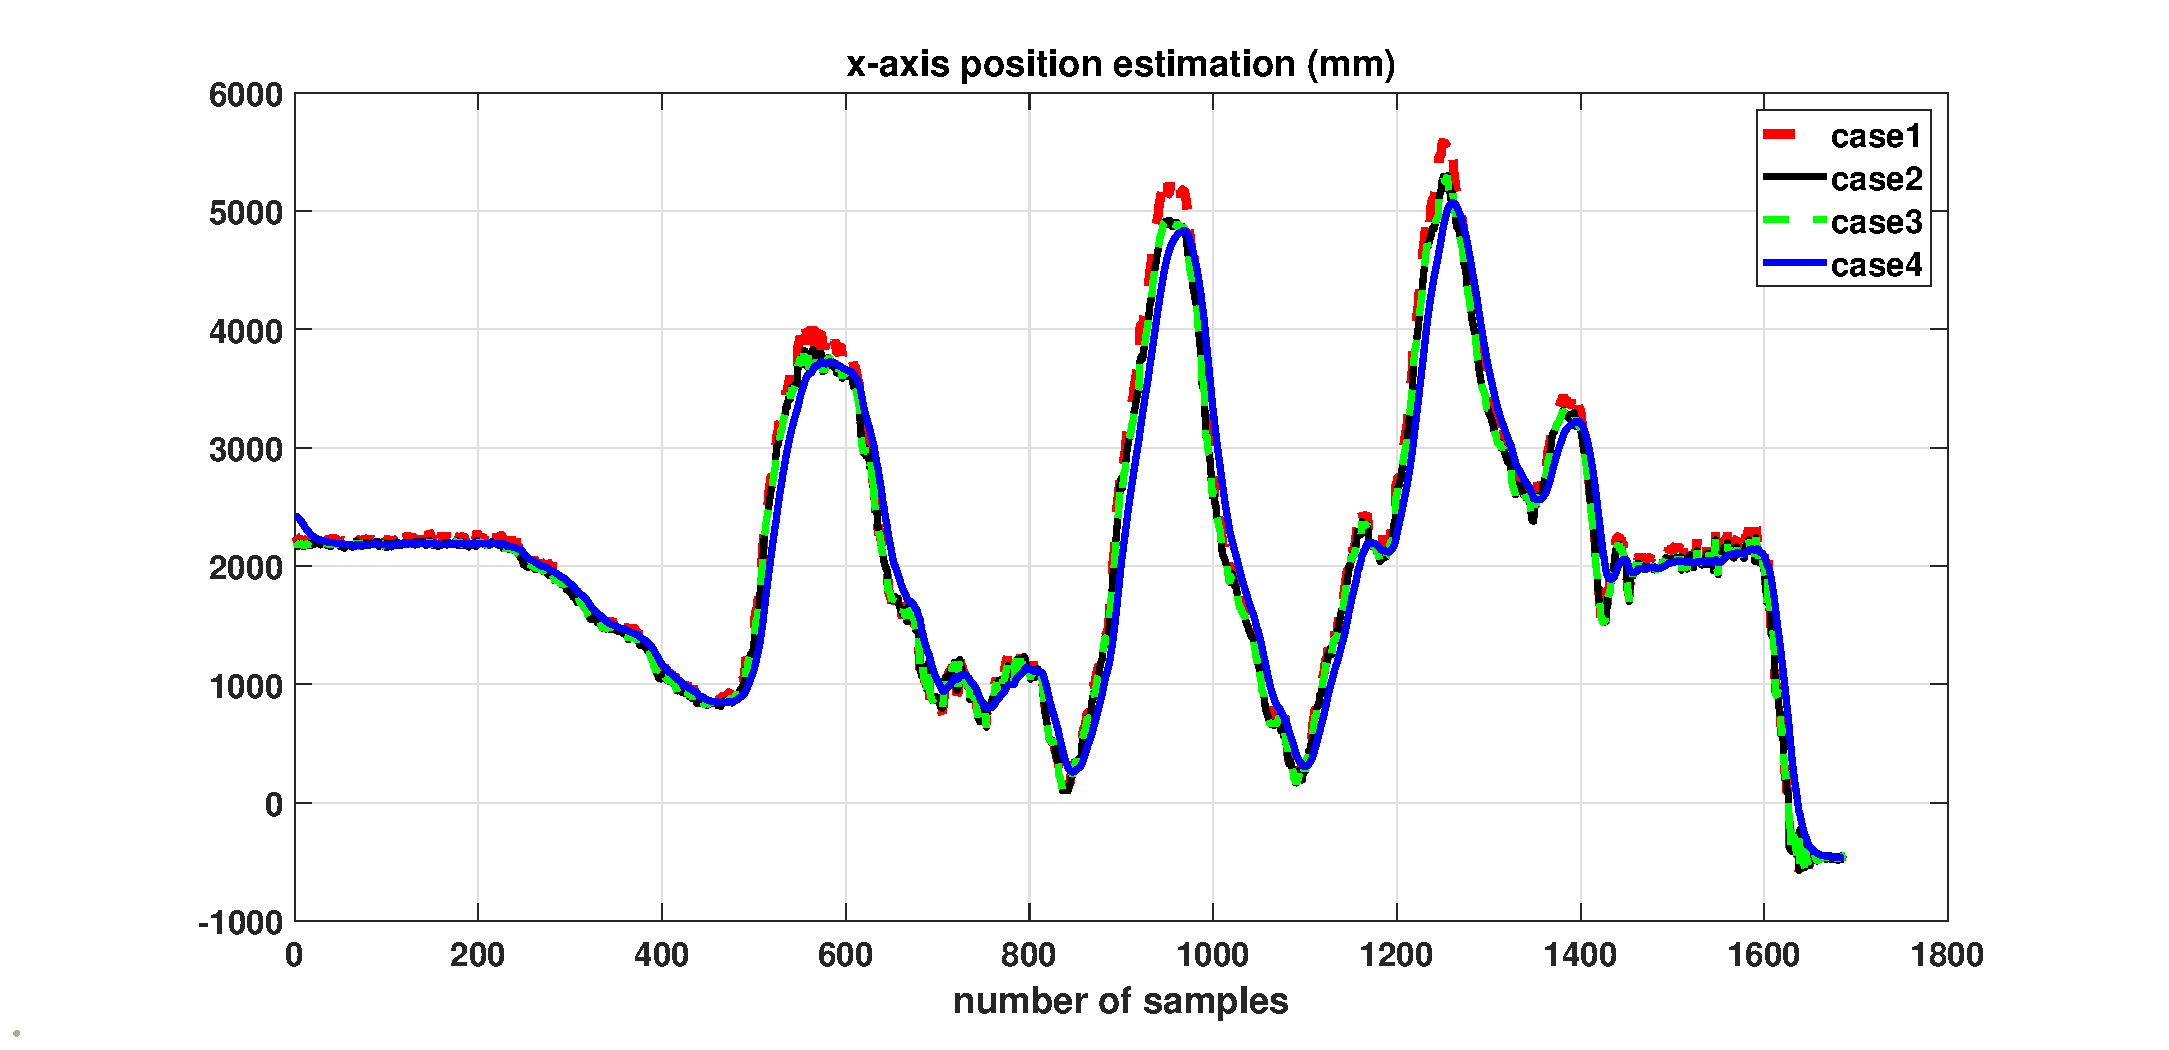
\includegraphics[scale=0.4]{Pics/Fig_logged/pos_x.eps}
\caption{Estimated x-axis position. There is not huge difference on the x-axis position estimation between the cases.}
\label{Fig_logged_01}
\end{figure}

\begin{figure}[thpb]
\centering
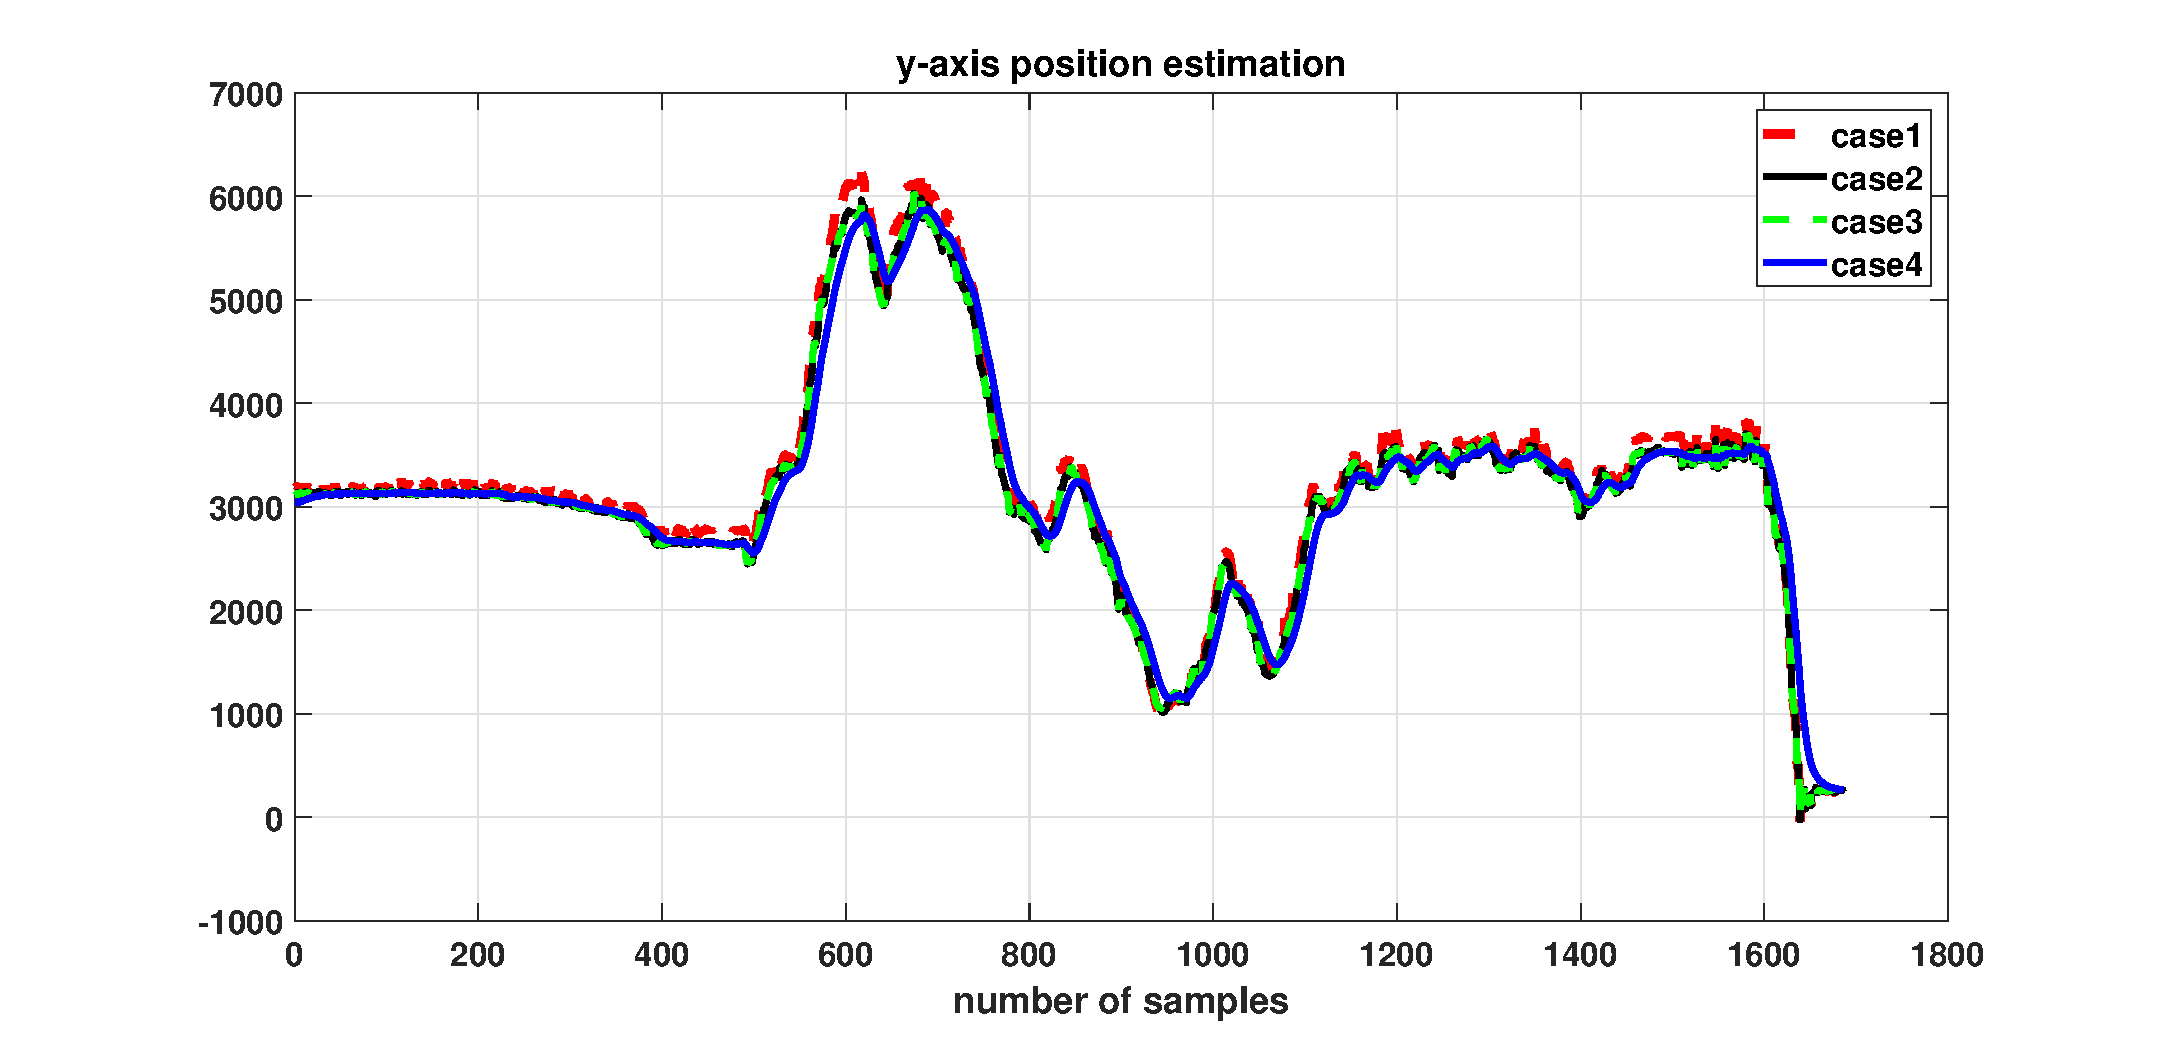
\includegraphics[scale=0.4]{Pics/Fig_logged/pos_y.eps}
\caption{Estimated y-axis position. There is not huge difference on the y-axis position estimation between the cases.}
\label{Fig_logged_02}
\end{figure}

\begin{figure}[thpb]
\centering
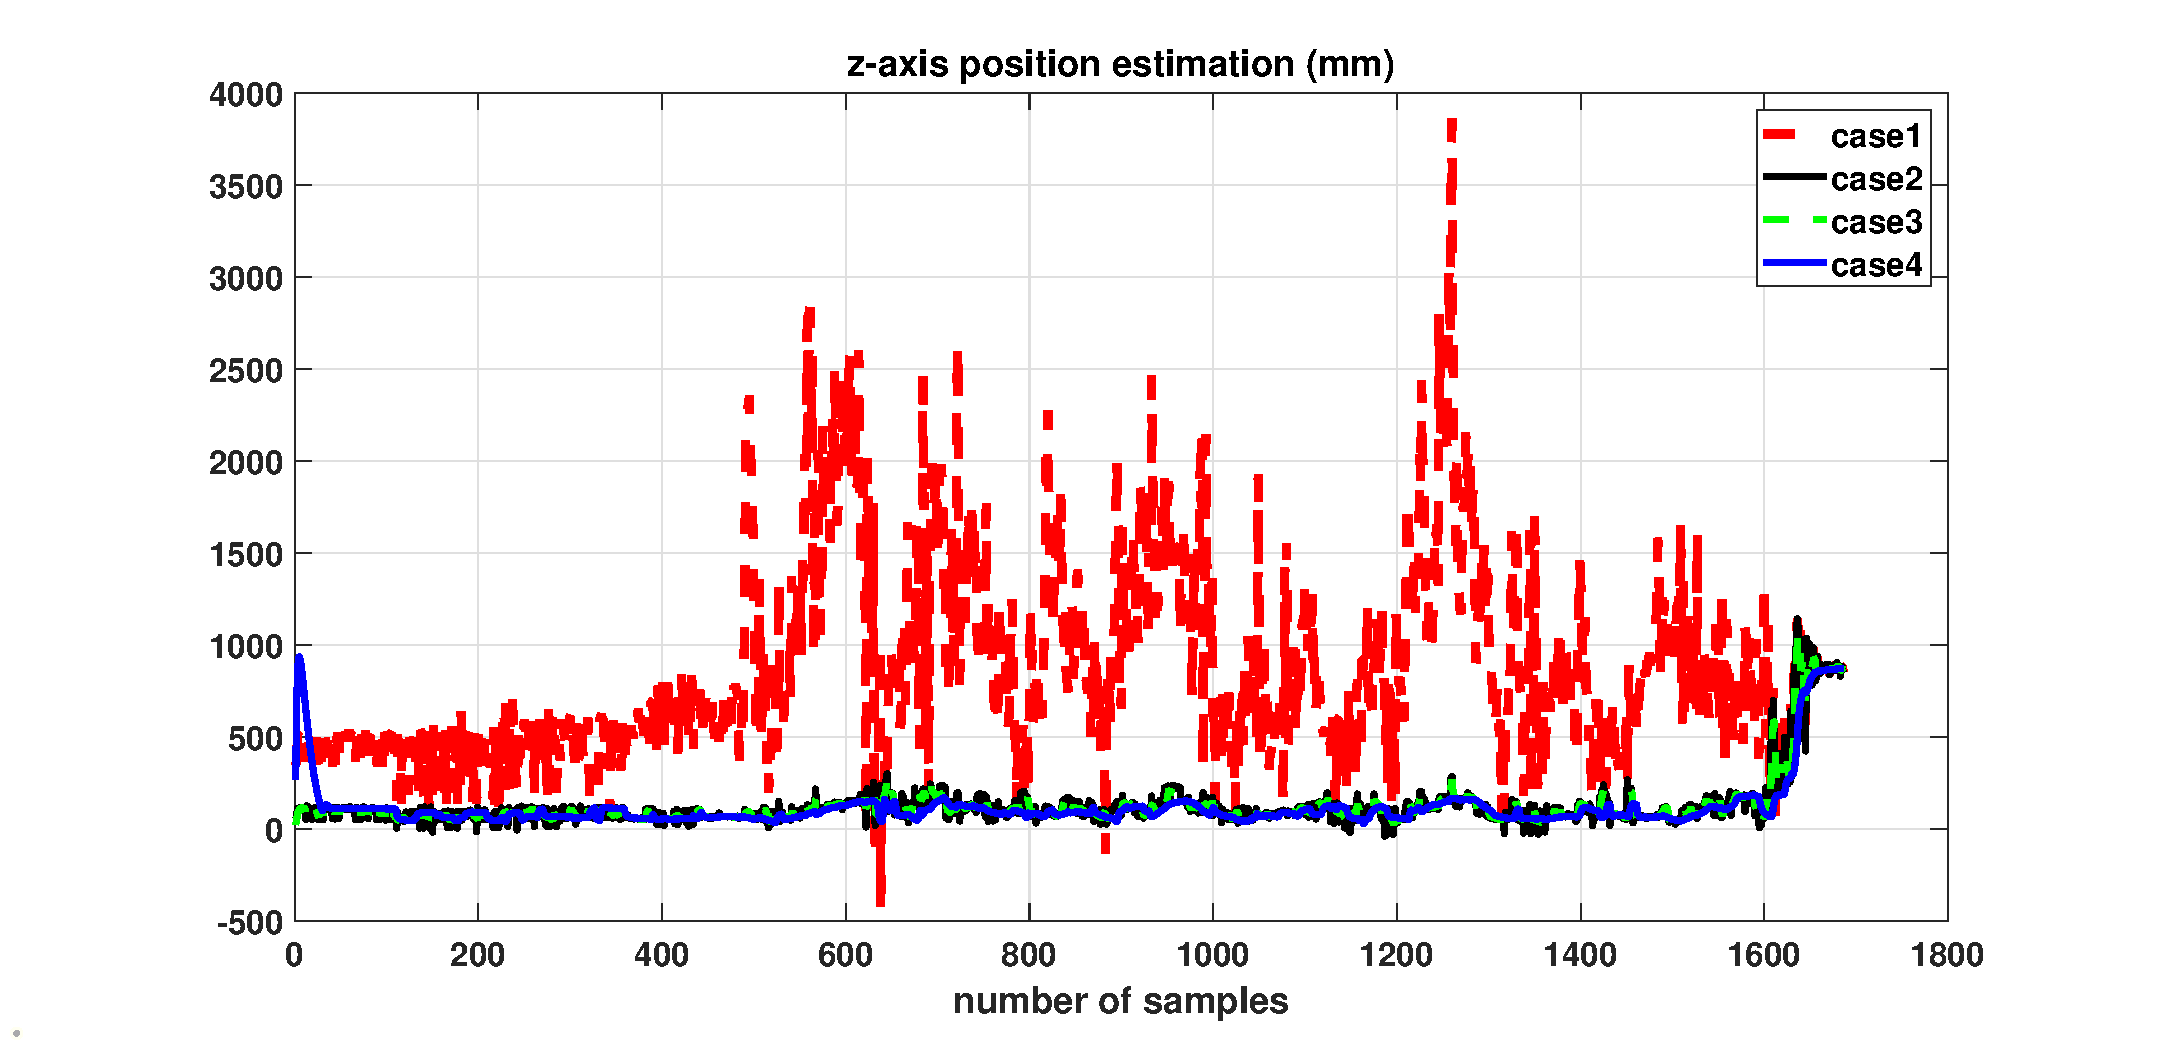
\includegraphics[scale=0.4]{Pics/Fig_logged/pos_z.eps}
\caption{Estimated z-axis position. As can be seen, tuning the learning rate and the breaking point parameters of the GD algorithm has the most effect on having good results on z-axis position estimation. We know that the correct z-axis position is something around 20cm.}
\label{Fig_logged_03}
\end{figure}

\begin{figure}[thpb]
\centering
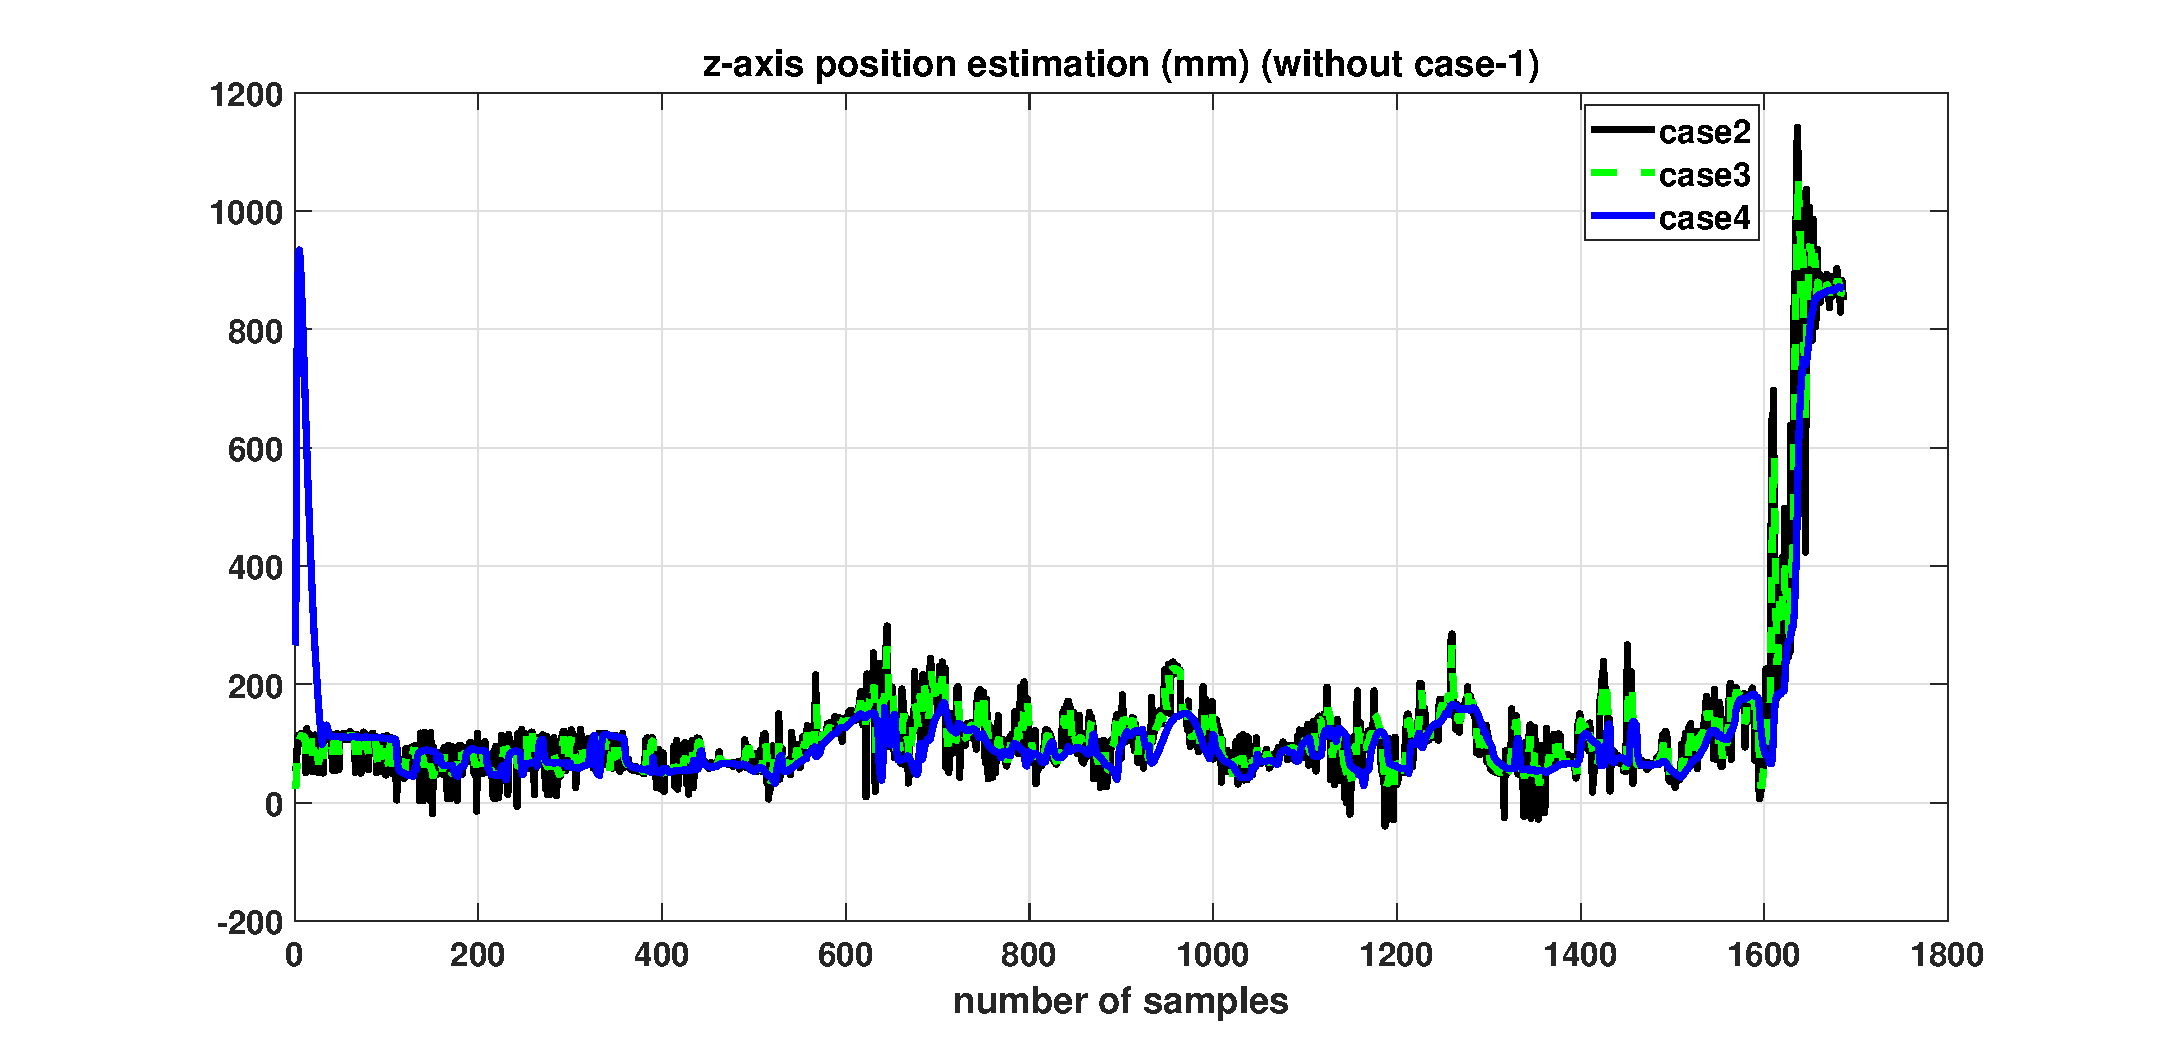
\includegraphics[scale=0.4]{Pics/Fig_logged/pos_z1.eps}
\caption{Estimated z-axis position, without case-1. The effect of using KFs over the distance measurements as well as the z-axis position estimation is obvious on smoothing the z-axis position estimation. Also, there is an initial converging phase for the operation of the linear KF on the distance measurements. We know that the correct z-axis position is something around 20cm.}
\label{Fig_logged_04}
\end{figure}

\begin{figure}[thpb]
\centering
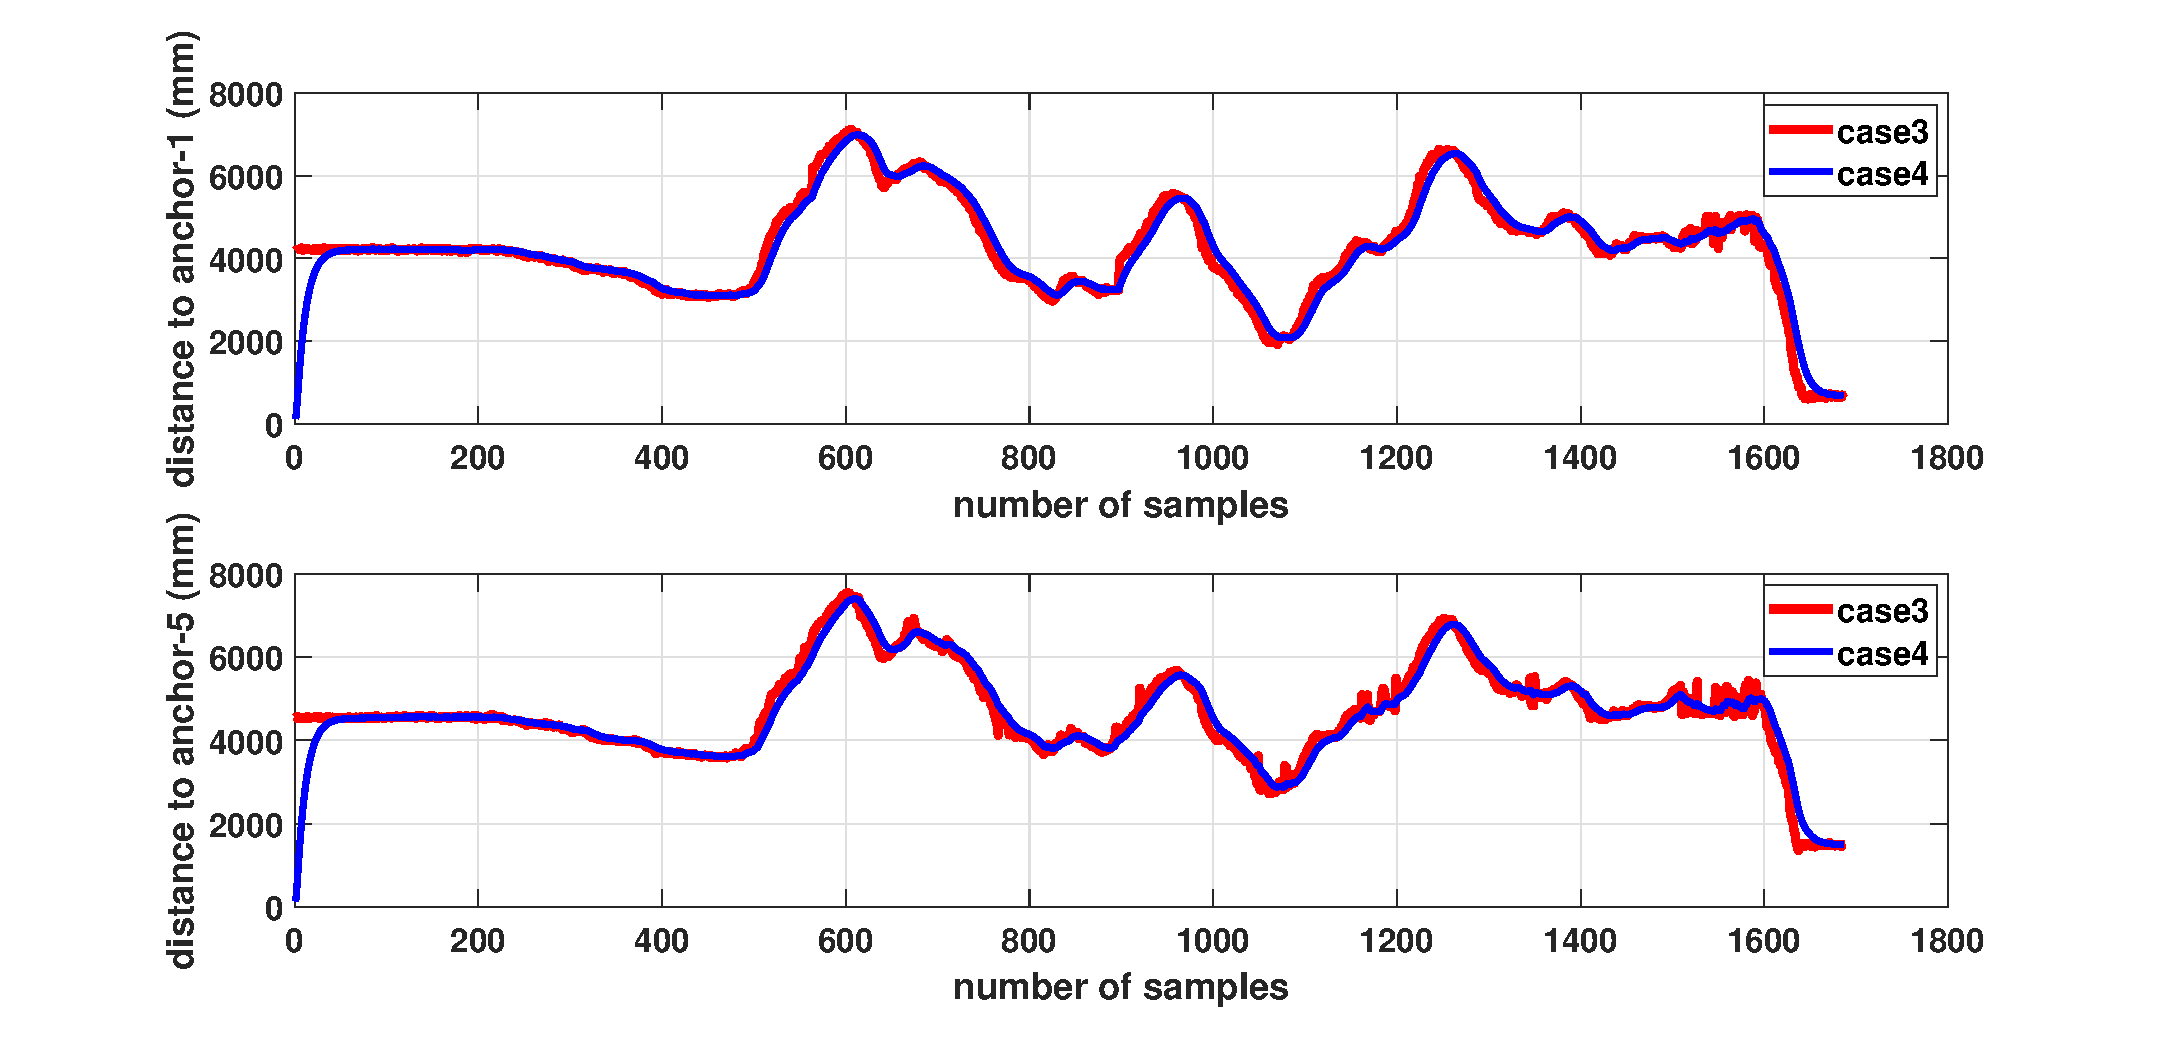
\includegraphics[scale=0.4]{Pics/Fig_logged/dist_15.eps}
\caption{Measured distances to the anchors on the first column. Using the KF on the measured distances, we have more smooth measurements.}
\label{Fig_logged_05}
\end{figure}

\begin{figure}[thpb]
\centering
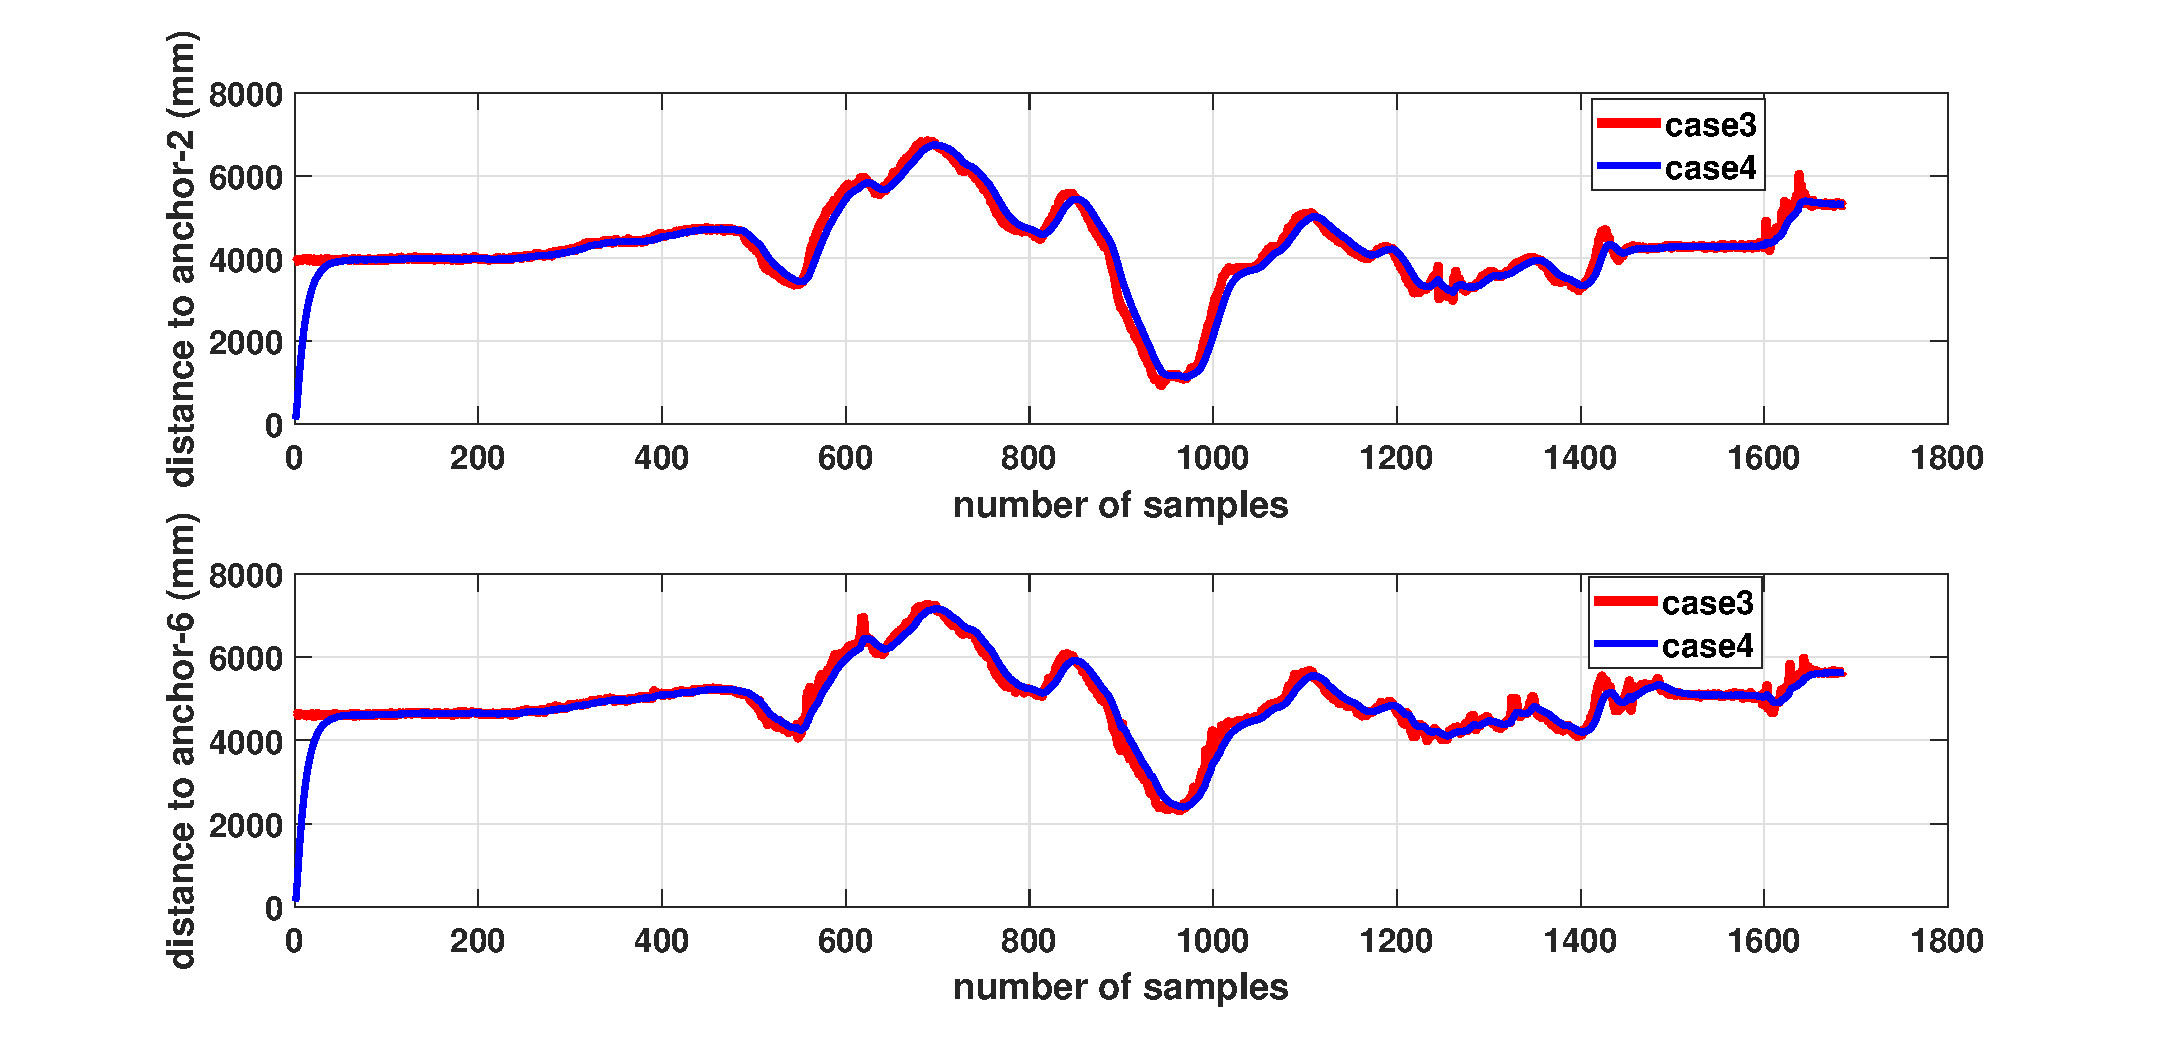
\includegraphics[scale=0.4]{Pics/Fig_logged/dist_26.eps}
\caption{Measured distances to the anchors on the second column. Using the KF on the measured distances, we have more smooth measurements.}
\label{Fig_logged_06}
\end{figure}

\begin{figure}[thpb]
\centering
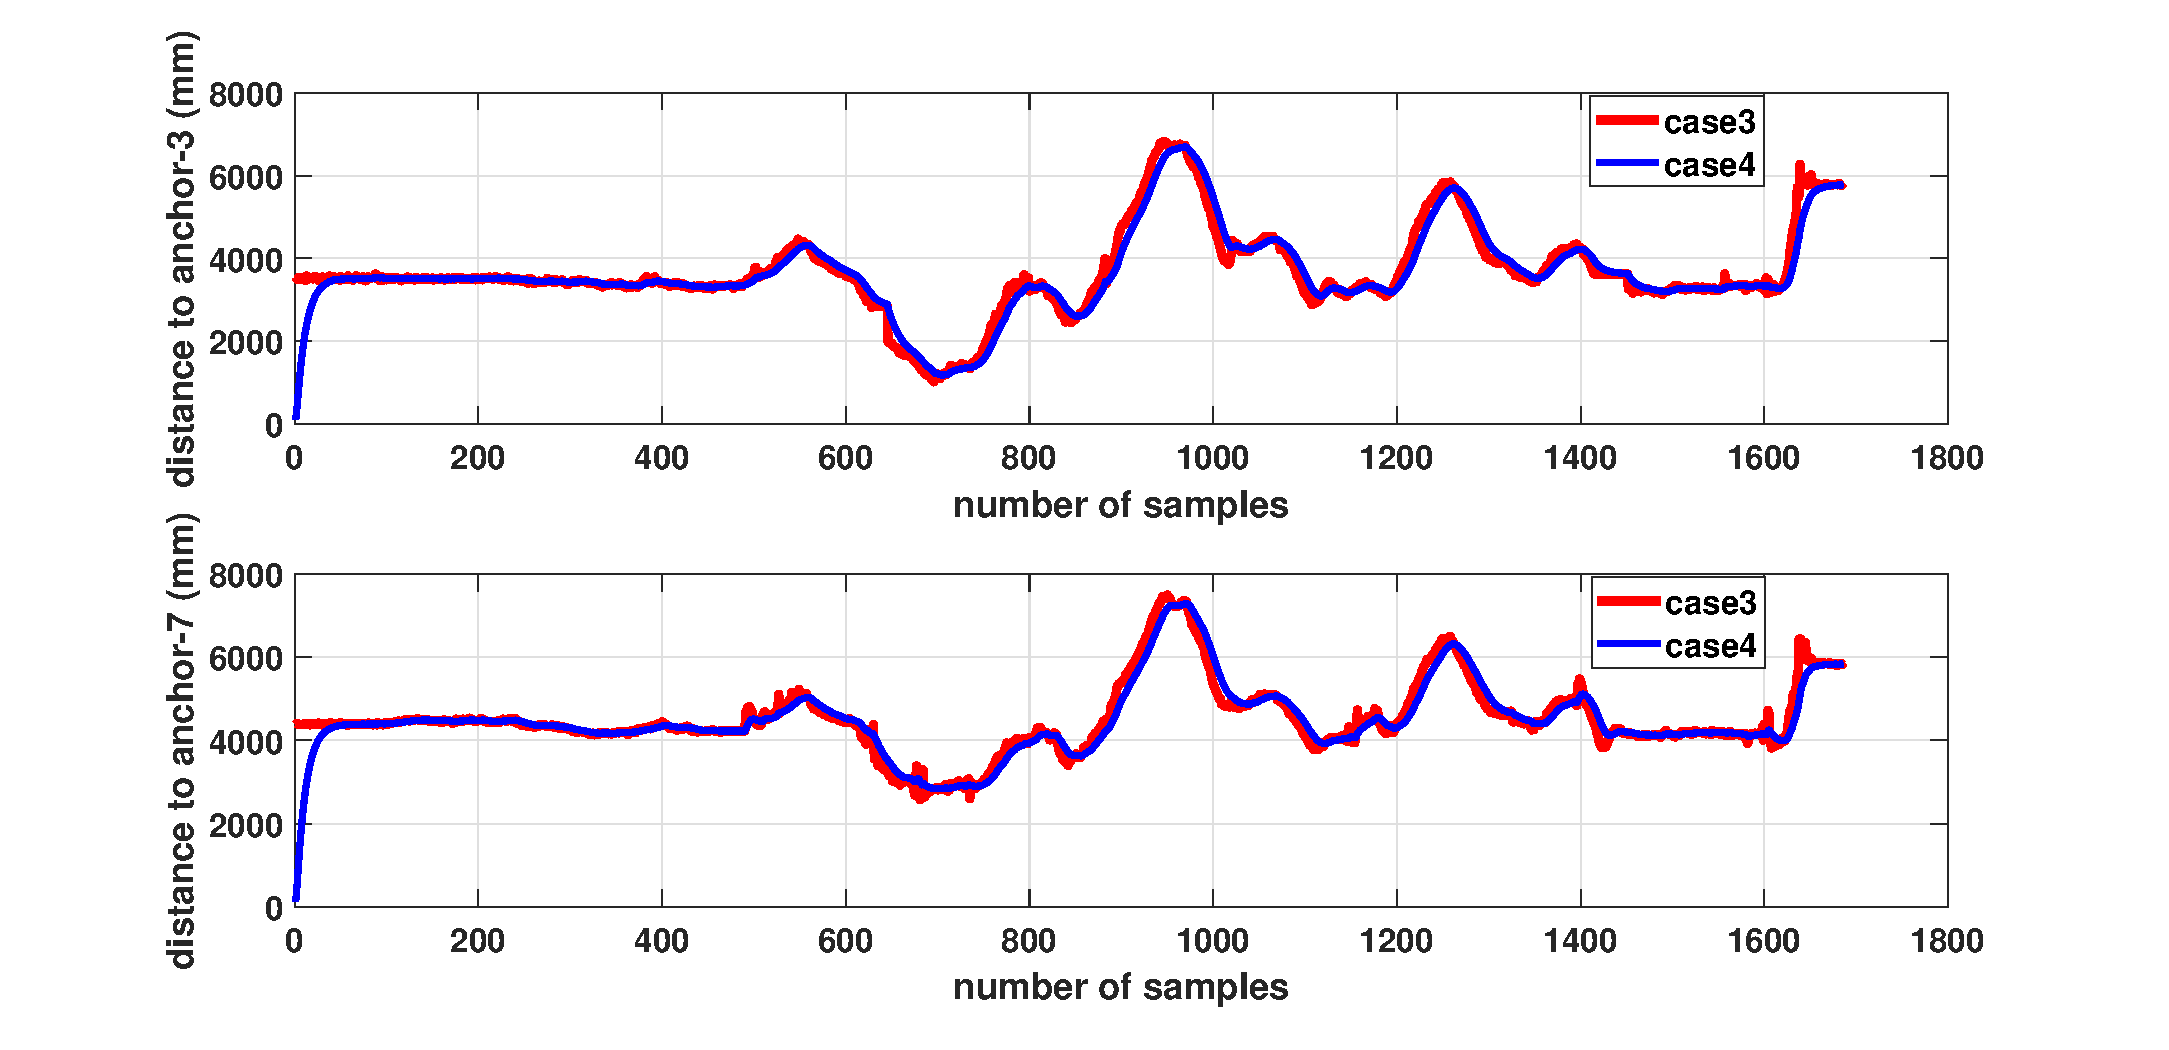
\includegraphics[scale=0.4]{Pics/Fig_logged/dist_37.eps}
\caption{Measured distances to the anchors on the third column. Using the KF on the measured distances, we have more smooth measurements.}
\label{Fig_logged_07}
\end{figure}

\begin{figure}[thpb]
\centering
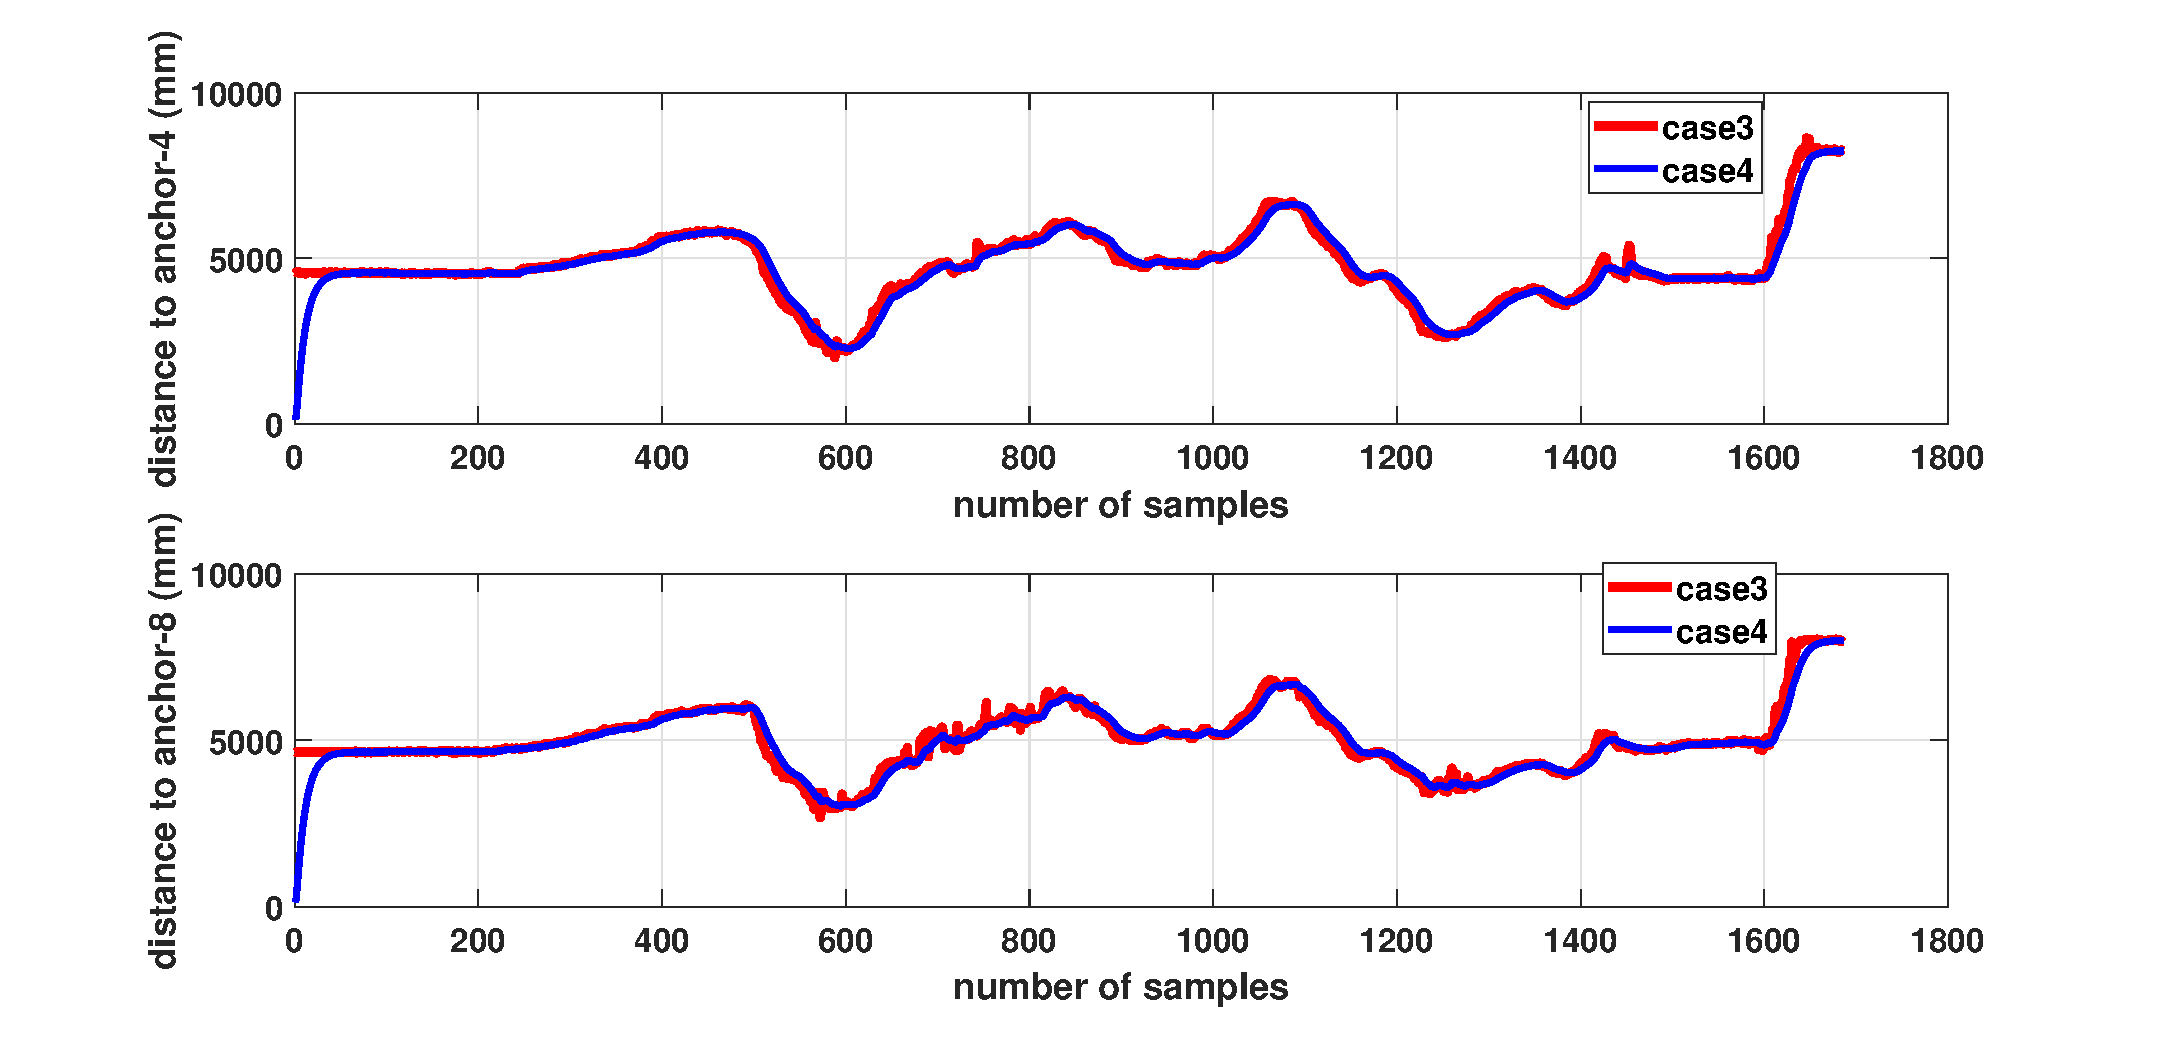
\includegraphics[scale=0.4]{Pics/Fig_logged/dist_48.eps}
\caption{Measured distances to the anchors on the fourth column. Using the KF on the measured distances, we have more smooth measurements.}
\label{Fig_logged_08}
\end{figure}

\newpage
\subsection{A GD algorithm for absolute velocity estimation in the UWB positioning system}
Recalling the estimated distance of the UWB tag to the $i$th anchor in the UWB positioning system, and also the estimated 3D position of the UWB tag using the algorithm presented in Section 3.3 and Section 3.5, the euclidean distance of the tag to the $i$th anchor can be written as follows
\begin{equation} \label{Eq_AbsVel_01}
(\hat{x}(t) - x_i)^2 + (\hat{y}(t) - y_i)^2 + (\hat{z}(t) - z_i)^2 = \hat{d}_i(t)^2 + \delta_i(t) \;,
\end{equation}
where $\hat{p}(t) = [\hat{x}(t);\hat{y}(t);\hat{z}(t)] \in \mathbb{R}^3$ is the estimated 3D position of the tag, $d_i(t) \in \mathbb{R}^+$ is the estimated distance from the tag to the $i$th anchor and $\delta_i(t) \in \mathbb{R}$ is the error associated to the whole estimation process (including the distance and 3D position estimations) at time $t$.
By performing a time derivation over the above equation, one would have
\begin{equation} \label{Eq_AbsVel_02}
\dot{\hat{x}}(t) (\hat{x}(t) - x_i) + \dot{\hat{y}}(t) (\hat{y}(t) - y_i) + \dot{\hat{z}}(t) (\hat{z}(t) - z_i) = \dot{\hat{d}}_i(t) \hat{d}_i(t) + \frac{1}{2} \dot{\delta}_i(t) \;.
\end{equation}
Here, $\dot{\hat{d}}_i(t) \in \mathbb{R}$ and $\dot{\delta}_i(t) \in \mathbb{R}$ are the time-derivatives of the $\hat{d}_i$ and $\delta_i$.
Moreover, $\dot{\hat{p}}(t) = [\dot{\hat{x}}(t);\dot{\hat{y}}(t);\dot{\hat{z}}(t)] \in \mathbb{R}^3$ is the time-derivative of the estimated 3D position of the tag.
Meanwhile, one may consider $\dot{\hat{p}}(t) \approx \hat{\dot{p}}(t) = \hat{v}(t)$, where $\hat{v}(t) \in \mathbb{R}^3$ is the estimated absolute 3D velocity of the UWB tag in the local frame of UWB positioning system, at time $t$.

By merging the equation in (\ref{Eq_AbsVel_02}) for all of the anchors ($i \in [1,n]$), one would have $A_v \hat{v} = B_v$, where 
\begin{equation}\label{Eq_AbsVel_03}
A_v = \left[\begin{matrix}
 (\hat{x}(t) - x_1) & (\hat{y}(t) - y_1) & (\hat{z}(t) - z_1) \\
 (\hat{x}(t) - x_2) & (\hat{y}(t) - y_2) & (\hat{z}(t) - z_2) \\
 (\hat{x}(t) - x_3) & (\hat{y}(t) - y_3) & (\hat{z}(t) - z_3) \\
\vdots & \vdots & \vdots  \\
 (\hat{x}(t) - x_n) & (\hat{y}(t) - y_n) & (\hat{z}(t) - z_n) \\
\end{matrix}\right] \in \mathbb{R}^{n \times 3}
\end{equation}
and
\begin{equation} \label{Eq_AbsVel_04}
B_v = \left[\begin{matrix}
\dot{\hat{d}}_1(t) \hat{d}_1(t) + \frac{1}{2} \dot{\delta}_1(t) \\
\dot{\hat{d}}_2(t) \hat{d}_2(t) + \frac{1}{2} \dot{\delta}_2(t) \\
\dot{\hat{d}}_3(t) \hat{d}_3(t) + \frac{1}{2} \dot{\delta}_3(t) \\
\vdots \\
\dot{\hat{d}}_n(t) \hat{d}_n(t) + \frac{1}{2} \dot{\delta}_n(t) \\
\end{matrix}\right] \in \mathbb{R}^{n \times 1} \;.
\end{equation}
Here $n=8$, as we are using eight anchors in the UWB positioning system. 
Obviously, the same GD algorithm used in Section 3.2 and Section 3.3 for solving the linear equations $A\hat{X} = B$ and $A_2 \hat{X}_2 = B_2$ can be incorporated for solving $A_v \hat{v} = B_v$. 
The experimental results for evaluating the performance of the proposed velocity estimation solution is provided in Section 4.6. \\

\textbf{Remark-9}. As seen in the right-hand side of (\ref{Eq_AbsVel_02}), the time-derivatives of the estimated distances from the tag to all of the anchors as well as the associated estimation errors (i.e. $\delta_i$) are required for the proposed velocity estimation algorithm. 
To deal with this issue, a sliding-mode differentiator has been utilized. 
For a generic scalar variable $r \in \mathbb{R}$, its time-derivative can be computed as \cite{Slid_Obs1,Slid_Obs}
\begin{equation} \label{Eq_AbsVel_05}
\dot{r} = \nu \;,
\end{equation}
where
\begin{equation} \label{Eq_AbsVel_06}
\begin{split}
\dot{q} &= \nu \\
\nu &= -k_1 |q - r|^{1/2} \; sgn(q - r) + \nu_1 \\
\dot{\nu}_1 &= -k_2 \; sgn(q - r)
\end{split}
\end{equation}
with $k_1>0$ and $k_2>0$ are two constant parameters and $sgn(.)$ is the signum function \cite{Slid_Obs1,Slid_Obs}. 
This lemma has been already used in several research investigations \cite{Ali_AMFC01,Ali_AMFC02,Ali_VelEst}. 
In the current implementations, the corresponding gains are tuned as $k_1 = 10.0$ and $k_2=1.0$. \\

\textbf{Remark-10}. Considering the proposed solutions in Section 3, the scheme of UWB indoor positioning system is depicted in Fig. \ref{Fig_scheme_total}

\begin{figure}[thpb]
\centering
\includegraphics[scale=0.4]{Pics/UWB_position_velocity_estimations.jpg}
\caption{The entire scheme of the UWB indoor positioning system for 3D position and velocity estimations.}
\label{Fig_scheme_total}
\end{figure}



\newpage
\subsection{Relative velocity computation}
A UDP connection over WiFi network is provided between the embedded modules attached to the UWB tags, so as to transmit to local velocity of each mobile agent to the other one. 
This information would be used later on for estimating the relative position (a vector) of the two moving agents (i.e. drones).
Note that the relative position among the agents in a swarm of drones is a most to compute the consensus errors required in decentralized \textit{cooperative controller} at each agent.

The rotation matrix at each drone should be considered to compute the relative velocity vector of each mobile agent (i.e. drone) in a local frame in the environment (and not in the body frame of the drone).

(Under development)


\subsection{Configuration}
In the current indoor localization system, there are 8 anchors located at the points of a cube. 
It is found that the update rate of the estimated position is slow, when the anchors are the initiators in the ranging process to the tag module. This is due to the collision occurred among the signals emitted from all the anchors and approaching the tag module.
Instead, if the tag module is the initiator of the ranging process with each of the anchors, the update rate for the localization system would be very fast. In this case, no signal collision is occurred.


\subsection{SEGGER Embedded Studio}
In order to write the codes in \textsf{C} language for implementation on DWM1001-dev module, we need to install \textsf{SEGGER Embedded Studio} software on a Windows operating system. The codes should be contained in sub-folders which in turn are included in a folder having all other required packages for compiling and uploading the codes into the module. This process can be understood completely by observing the examples provided by the DecaWave company. 

In addition, the software named as \textsf{SEGGER J-Flash Lite V6} should be installed for erasing and programming of the processor embedded in DWM1001-dev module. 

\subsection{Codes on DWM1001-dev module}
The codes are written in C language and provided on the following address in the local \textit{GitLab} repository at Humanitas:

\url{http://192.168.0.172/alzizou/testing-dwm1001-dev-modules/tree/master/Files_On_DWM1001dev}

\subsection{Codes on Raspberry PIs}
A ROS package in Python is provided for the embedded systems attached to each UWB tag modules, for handling the 3D localization and communicating with PX4. This ROS package includes the following nodes:
\begin{itemize}
    \item \textit{distance collection}: for communicating between the embedded board and the UWB tag module to collect distances to all of the anchors in the environment.
    \item \textit{localization}: for doing the 3D localization based on GD or ML algorithms and also implementing a new EKF outside of PX4.
    \item \textit{relative velocity}: for transmitting the local velocity of each moving agent (i.e. the drone) to the other moving agent.
    \item \textit{PX4 communication}: for communicating with PX4, including sending the estimated position, logging the filtered position and acceleration by EKF2, arming the drone, sending the target position, and changing the flight mode of the drone from manual to autonomous and vice-versa.
\end{itemize}

The separate packages are considered for Raspberry-Pi and NanoPi boards, as the name of serial ports in each of them is different.
The codes are written in Python language and provided on the following address in the local \textit{GitLab} repository at Humanitas:

\url{http://192.168.0.172/alzizou/testing-dwm1001-dev-modules/tree/master/Files_On_RPi}

\newpage
\section{Test Results}
The tests have been performed in two different cases with the stationary and moving tags.

\subsection{Stationary tag}
\subsubsection{Test the localization in $X-Y$ plane}
A digitized white-board is provided on the ground (i.e. in the plane of Z=0) in our lab. The location of one corner of the board is fixed on the ground and its position is known.
Then, the tag is placed on the white board on different grid. The estimated position in $X-Y$ plane using the UWB module is compared with the actual position of each grid. 
Note that since the estimated positions provided by the UWB system are varying with a certain amount of variance, the average values of the observed estimated position are reported.
The results are gathered in the excel file, which can be found in the HumanITAS Gitlab at this address: 
\url{http://192.168.0.172/alzizou/testing-dwm1001-dev-modules/tree/master/Report}
According to the test results, the average localization error in $X-Y$ plane is around 210mm.

\subsubsection{Test the localization in $Z$ axis}
For testing the localization in Z axis, a rod with the length of 2m is provided. The tag module is attached to four different places on the rod. Then, while the rod is fixed vertically on the ground in the middle of the lab, the $Z$ element of the estimated position at each of of the placements is observed and reported.
It has been observed that the localization error in $Z$ direction is increased by increasing the height of the placement. It varies from 200mm at the ground to about 1000mm at the height of 2m.
The results can be found in the excel file at the above address.
Improvements are on the way. 

\subsection{Moving tag}
A set of results for $X,Y,Z$ elements of the measured position of a moving tag module is presented here, while the tag was moving in $X-Y$ plane and its $Z$ axis position was constant. 
In the test, the tag module was located on a wheeled-chair and pushed in the lab in the direction of north-west in a local coordinate system. The data is gathered for the whole test, starting from a stationary state, moving toward north-west and reaching at the final stationary state. 
The results are depicted in Figure \ref{Fig_06} to Figure \ref{Fig_08}.
As can be seen:
\begin{enumerate}
    \item The variation of the measured values in $X-Y$ plane during the movement of the module is low. We can claim that the measured positions in $X-Y$ plane during the movement is almost as smooth as the measured positions in $X-Y$ plane while the tag is stationary. No harsh disruption in measurements is observed while the tag is moving.
    \item Although the Z position of the element is constant, the measured $Z$ position of the tag is changing according to its movement in $X-Y$ plane. It is a not-acceptable result. So, the localization algorithm should be improved to solve this issue.
    \item The variation of the measured positions in $X,Y,Z$ directions for the tag during the stationary states is very minor and the results are changing a little around their corresponding mean values. The achieved standard deviation of the measurements in $X,Y,Z$ directions are 10,8,6mm at the initial stationary state, respectively; these values are 12,12,9mm for the final stationary state, respectively.
\end{enumerate}
 
\begin{figure}[thpb]
\centering
\includegraphics[scale=0.7]{Pics/Test_MovingTag_X.PNG}
\caption{Measurement of the X position of the moving tag during test}
\label{Fig_06}
\end{figure}

\begin{figure}[thpb]
\centering
\includegraphics[scale=0.7]{Pics/Test_MovingTag_Y.PNG}
\caption{Measurement of the Y position of the moving tag during test}
\label{Fig_07}
\end{figure}

\begin{figure}[thpb]
\centering
\includegraphics[scale=0.9]{Pics/Test_MovingTag_Z.PNG}
\caption{Measurement of the Z position of the moving tag during test}
\label{Fig_08}
\end{figure}

\newpage
\subsection{Testing the EKF performance}
Here, the results are provided in Figure \ref{Fig_09} and Figure \ref{Fig_10} for testing the performance of the EKF provided by default in PX4 platform.
As can be seen, while the data measured by the UWB system is pretty clear, the filtered output by the EKF is not appropriate. Further improvements on the EKF are required.

\begin{figure}[thpb]
\centering
\includegraphics[scale=0.4]{Pics/EKF_Test_UWB.PNG}
\caption{UWB measured position for testing the EKF performance}
\label{Fig_09}
\end{figure}

\begin{figure}[thpb]
\centering
\includegraphics[scale=0.4]{Pics/EKF_Test_EKF.PNG}
\caption{EKF outputs for testing the EKF performance}
\label{Fig_10}
\end{figure}

\newpage
\subsection{Results for GD localization on the second representation of the problem}
As mentioned in Section 3.3, by implementing the GD solution on the second representation of the problem, more consistent results, specially for Z axis would be achieved. The results are presented below.

\begin{figure}[thpb]
\centering
\includegraphics[scale=0.16]{Pics/Improved_Results_03.JPG}
\caption{Improved results for the moving module by implementing the GD localization on the second representation of the localization problem.}
\label{Fig_11}
\end{figure}


\begin{figure}[thpb]
\centering
\includegraphics[scale=0.4]{Pics/Improved_Results_04_Moving_Module.JPG}
\caption{Improved results for the stationary module on the different locations in the area, by implementing the GD localization on the second representation of the localization problem.}
\label{Fig_12}
\end{figure}

\newpage
\subsection{Results for evaluation the KF outside PX4 presented in Section 3.5}
By incorporating two linear KFs on each distance measurements as well as the z-axis estimated position by the GD algorithm (with tuned learning rates as suggested in Section 3.5), several experiments have been done in HumanITAS office, while a drone was flying in manual mode at very low altitude.
The results are presented in Fig. \ref{Fig_KF_01} and Fig. \ref{Fig_KF_02}. As can be seen more smooth 3D positions are estimated for the drone flying in the x-y plane at around 200cm altitude. The measured distances are also more clear, inhabiting lower fluctuations. The frequency of the localization process is between 4-6Hz. 
Note that in the current drone, the UWB tag is located at the bottom of the drone, leading to some non line of sight distance measurements. This has been changed in the new design of the drone.
But, the outputs of EKF2 inside the PX4 are not following the estimated UWB positions. 

\begin{figure}[thpb]
\centering
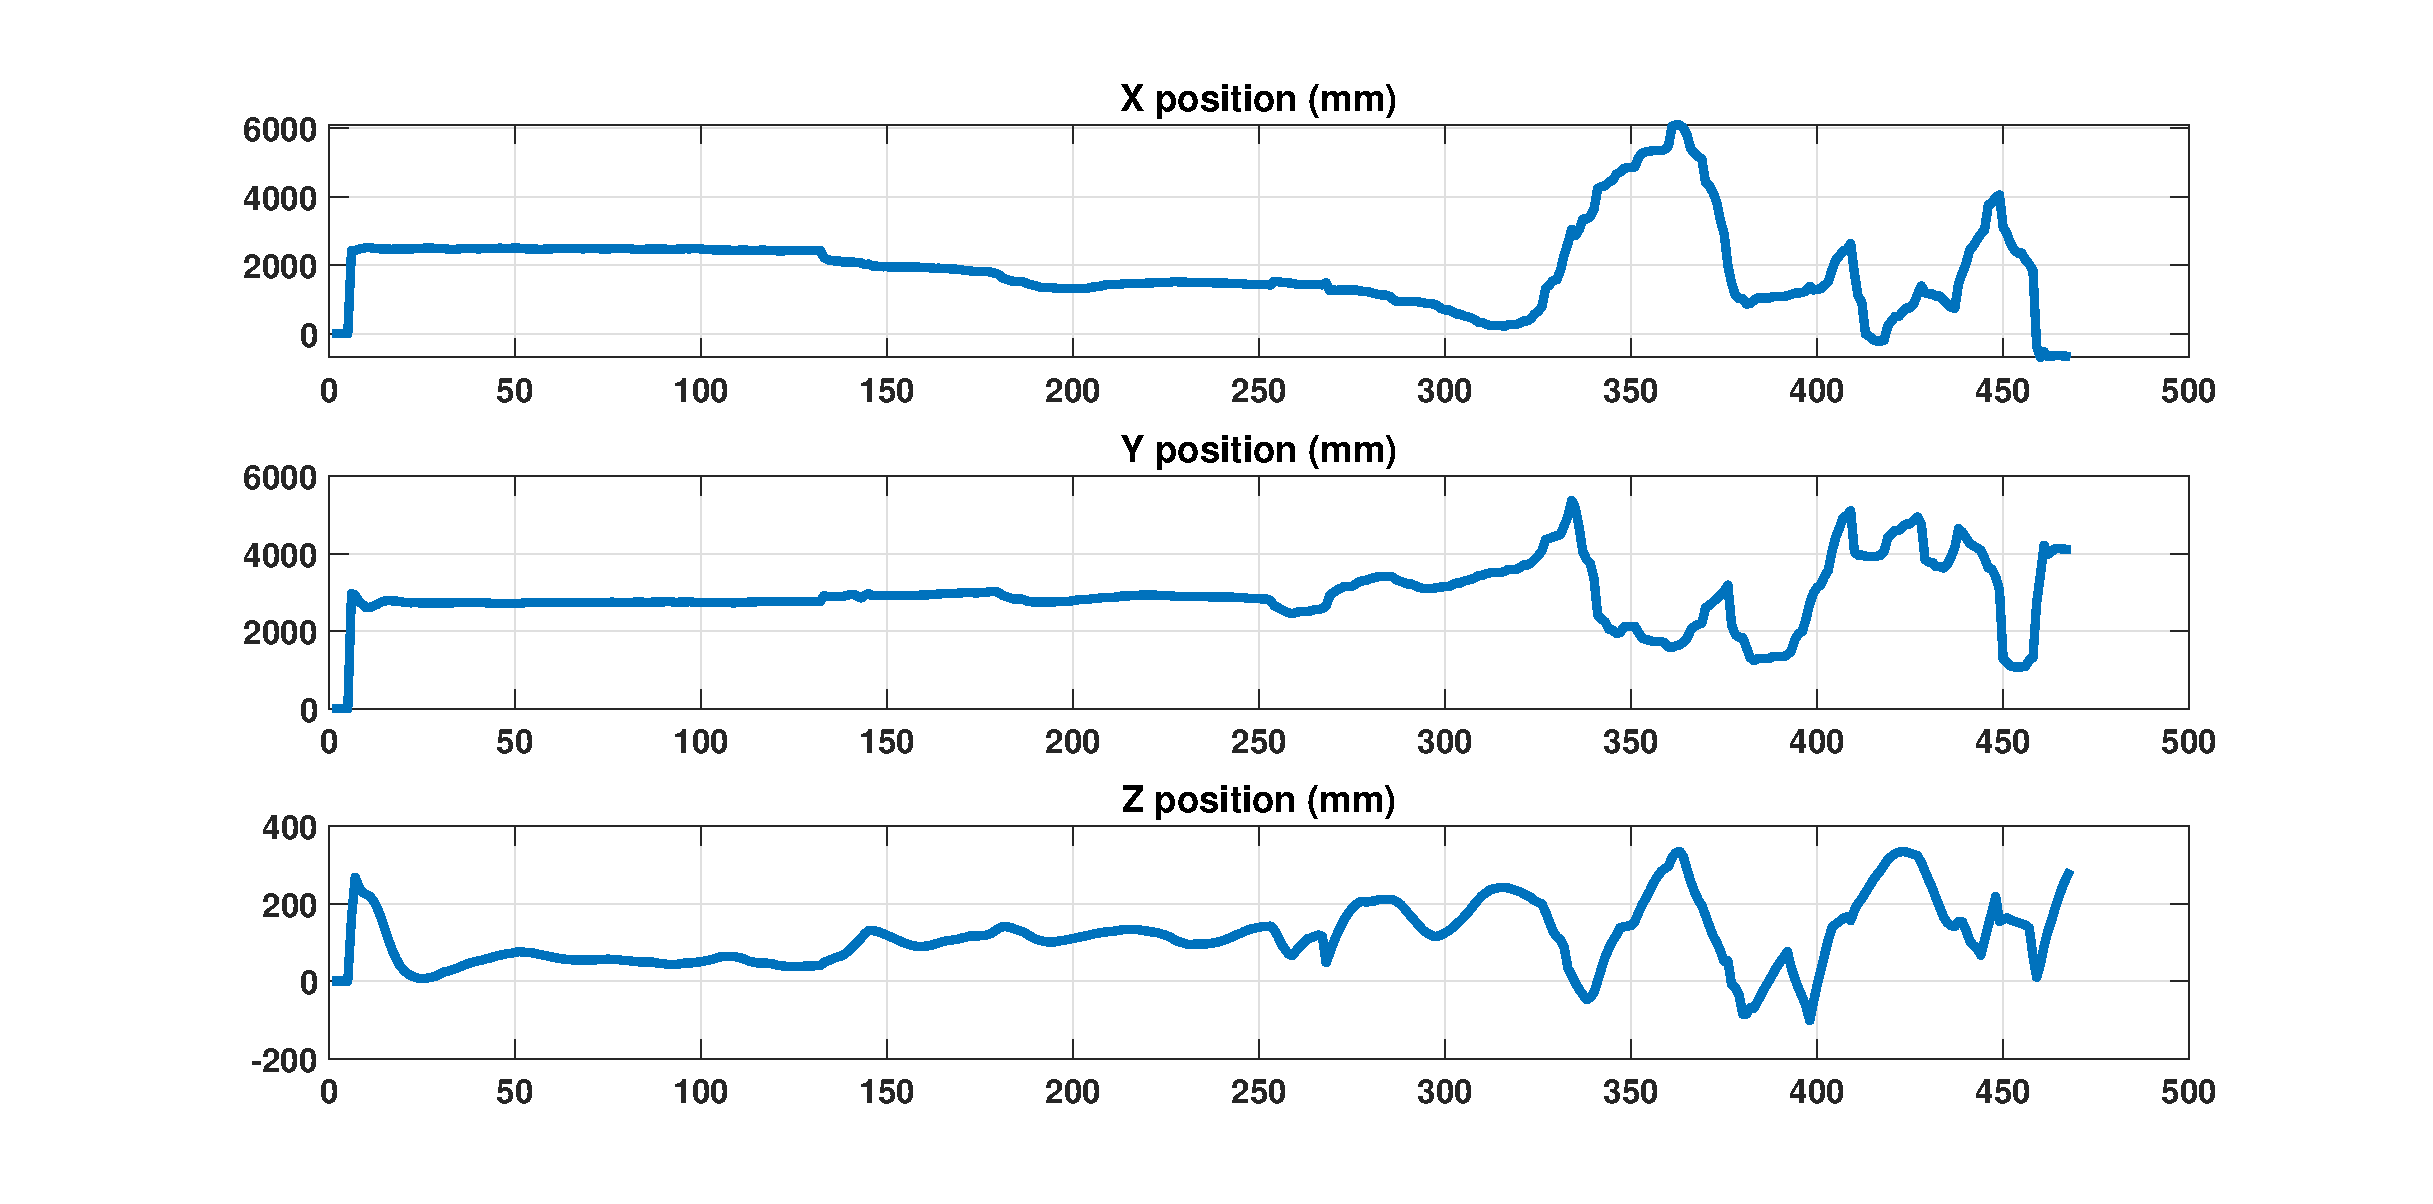
\includegraphics[scale=0.35]{Pics/UWB_Pos_20May_03.eps}
\caption{Improved results for the estimated 3D position by the UWB indoor localization system.}
\label{Fig_KF_01}
\end{figure}


\begin{figure}[thpb]
\centering
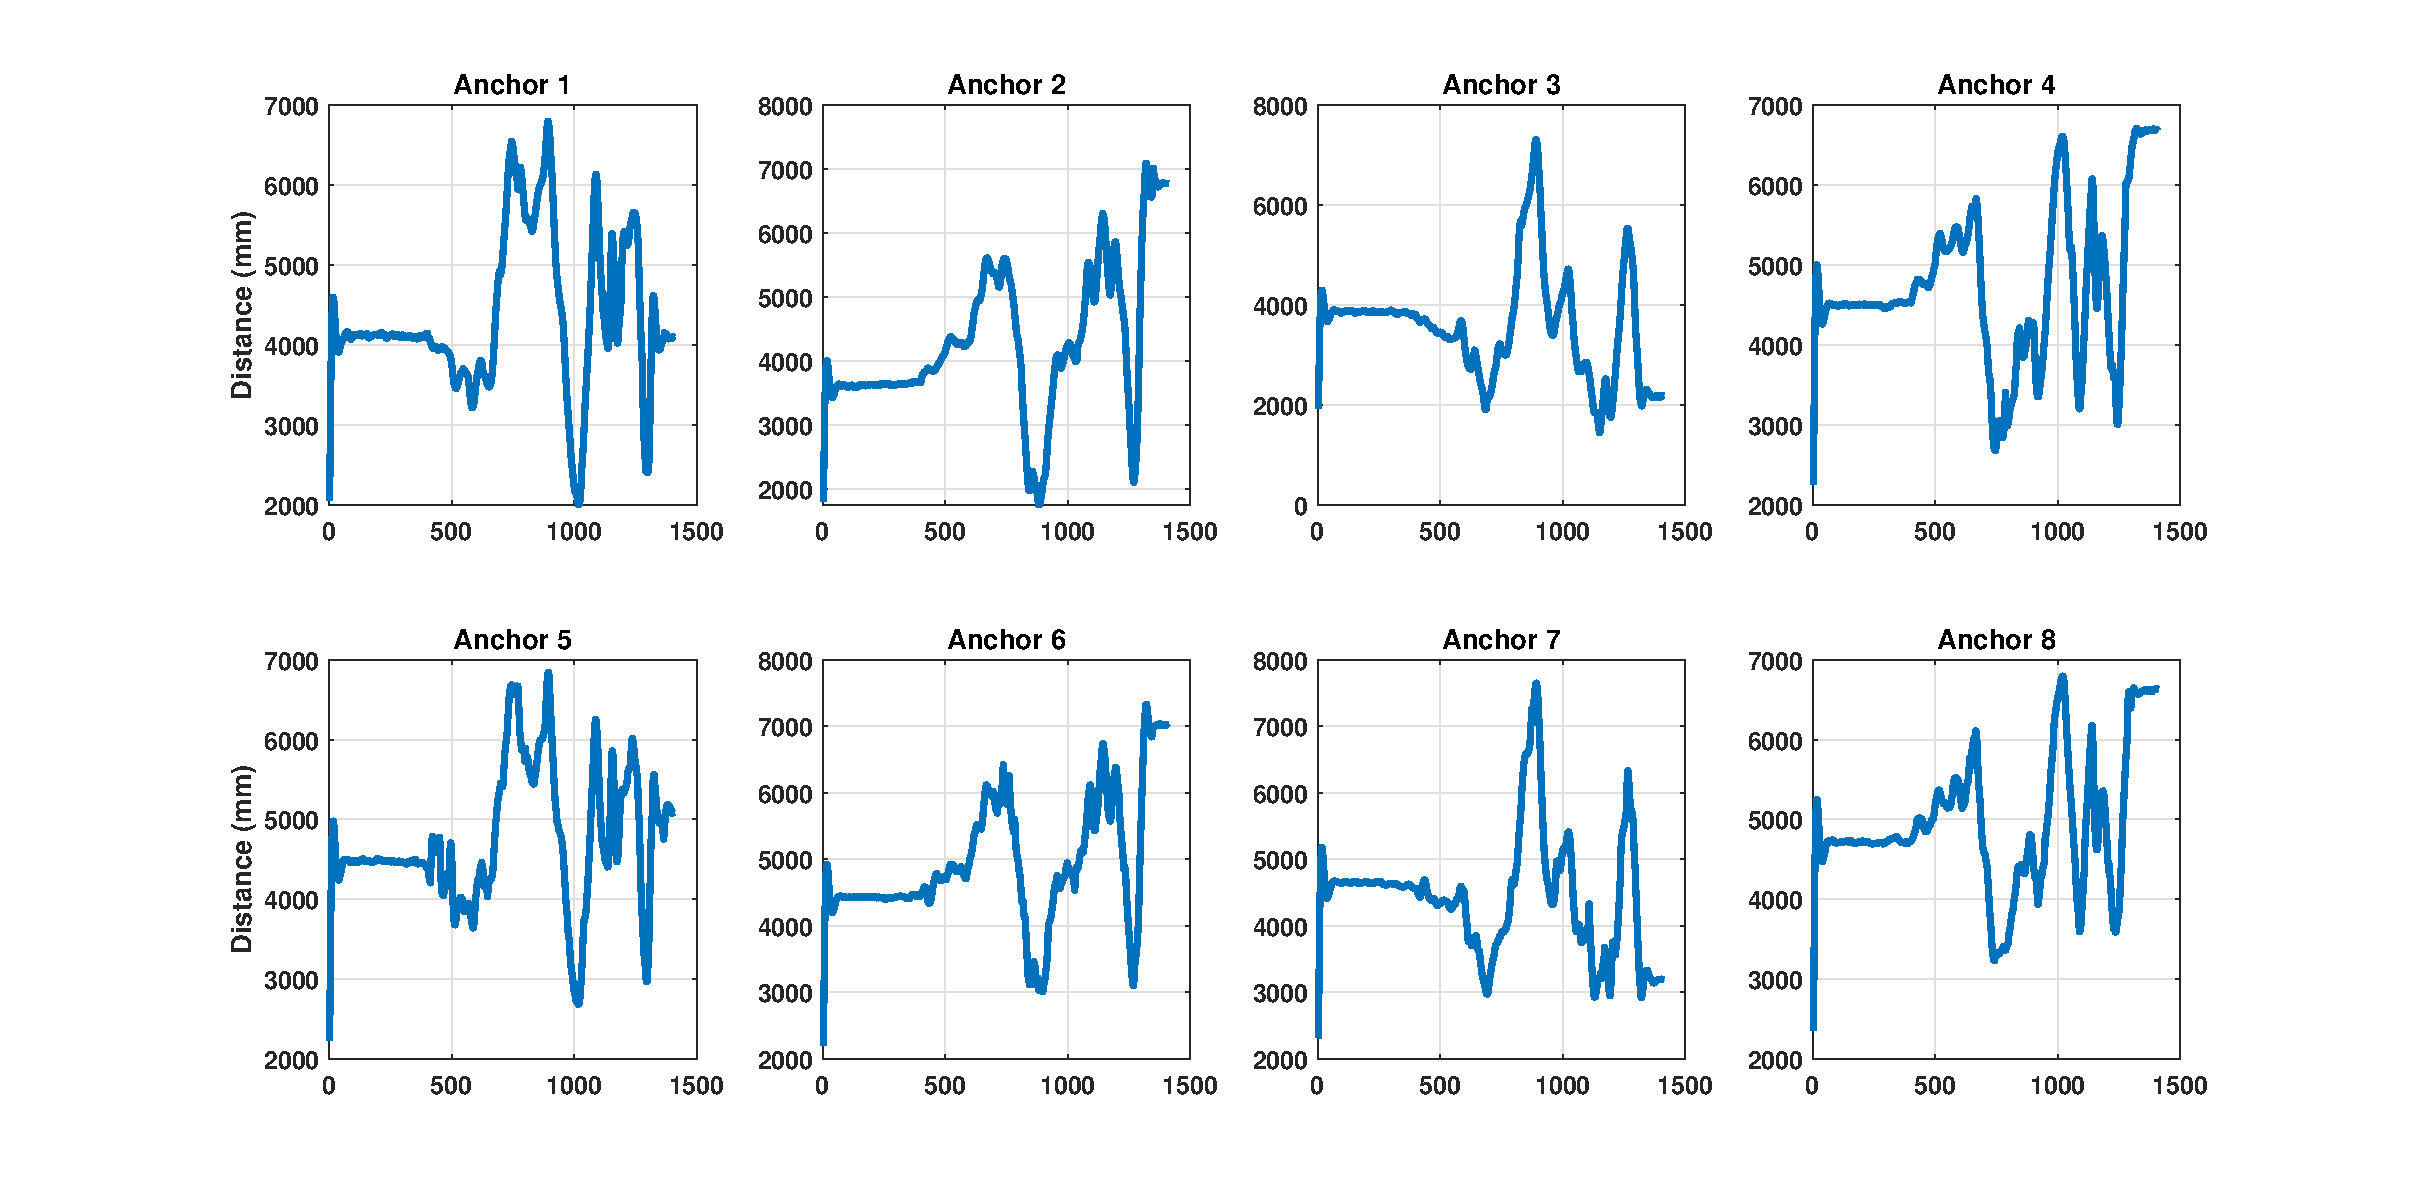
\includegraphics[scale=0.35]{Pics/UWB_Dist_20May_03.eps}
\caption{Improved results for the measured distances to the 8 anchors.}
\label{Fig_KF_02}
\end{figure}

\newpage
In order to see the capability of the UWB positioning system on z-axis position estimation, an experiment has been conducted in which the drone goes up manually to a height of around 1m and then decrease the altitude and do it again. The results for this test are presented in Fig. \ref{Fig_KF_03}.

\begin{figure}[thpb]
\centering
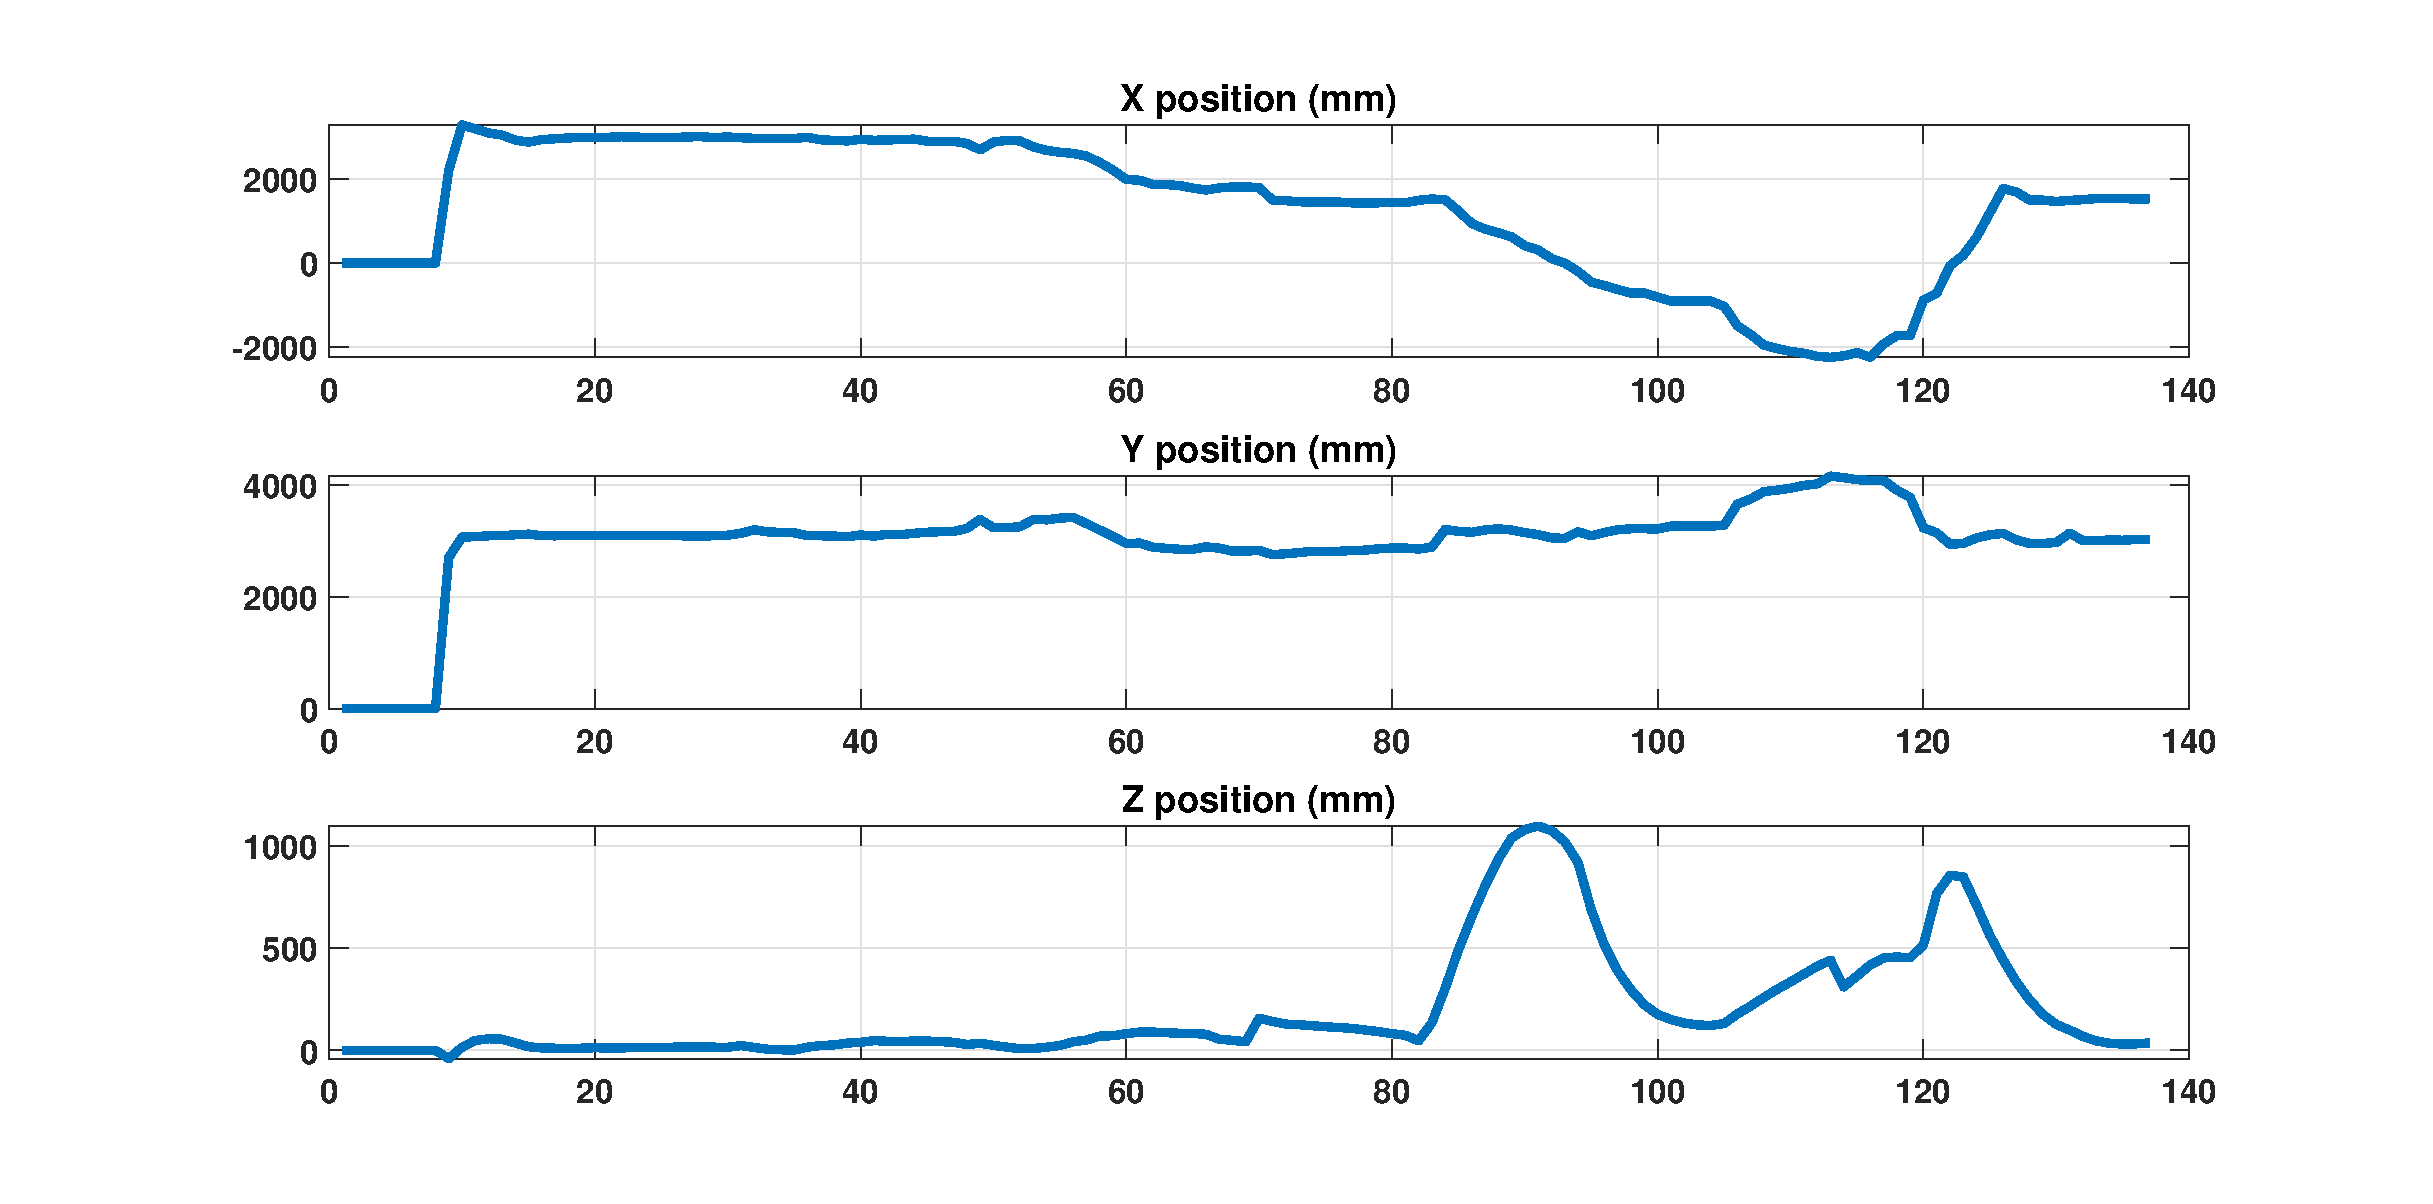
\includegraphics[scale=0.35]{Pics/UWB_Pos_21May_02.eps}
\caption{The results for experiment on the drone changing altitude.}
\label{Fig_KF_03}
\end{figure}

\newpage
\subsection{Experimental results for evaluating the performance of the velocity estimation solution proposed in Section 3.6}
In this section, the results for evaluating the 3D absolute velocity estimation solution in the UWB positioning system (as proposed in Section 3.6) are presented.
The results are gathered during the manual flight of one drone.
As can be seen the major issue at the current moment is that in some portions of the time (e.g. time window between 1.591392525e9 to 1.591392545e9 timestamps in the following figures) the acceleration measurements process is hanged (as seen in Fig. \ref{Fig_vel_03}) and the outputs of the EKF2 would not follow the estimated position and velocity (as seen in Fig. \ref{Fig_vel_04}). Using the data in Fig. \ref{Fig_vel_04}, it is not safe to go for an autonomous flight.

Moreover, the frequency of running the codes for collecting the distances to the anchors, position estimation and velocity estimation are depicted in Fig. \ref{Fig_vel_05} to Fig. \ref{Fig_vel_07}. 

\begin{figure}[thpb]
\centering
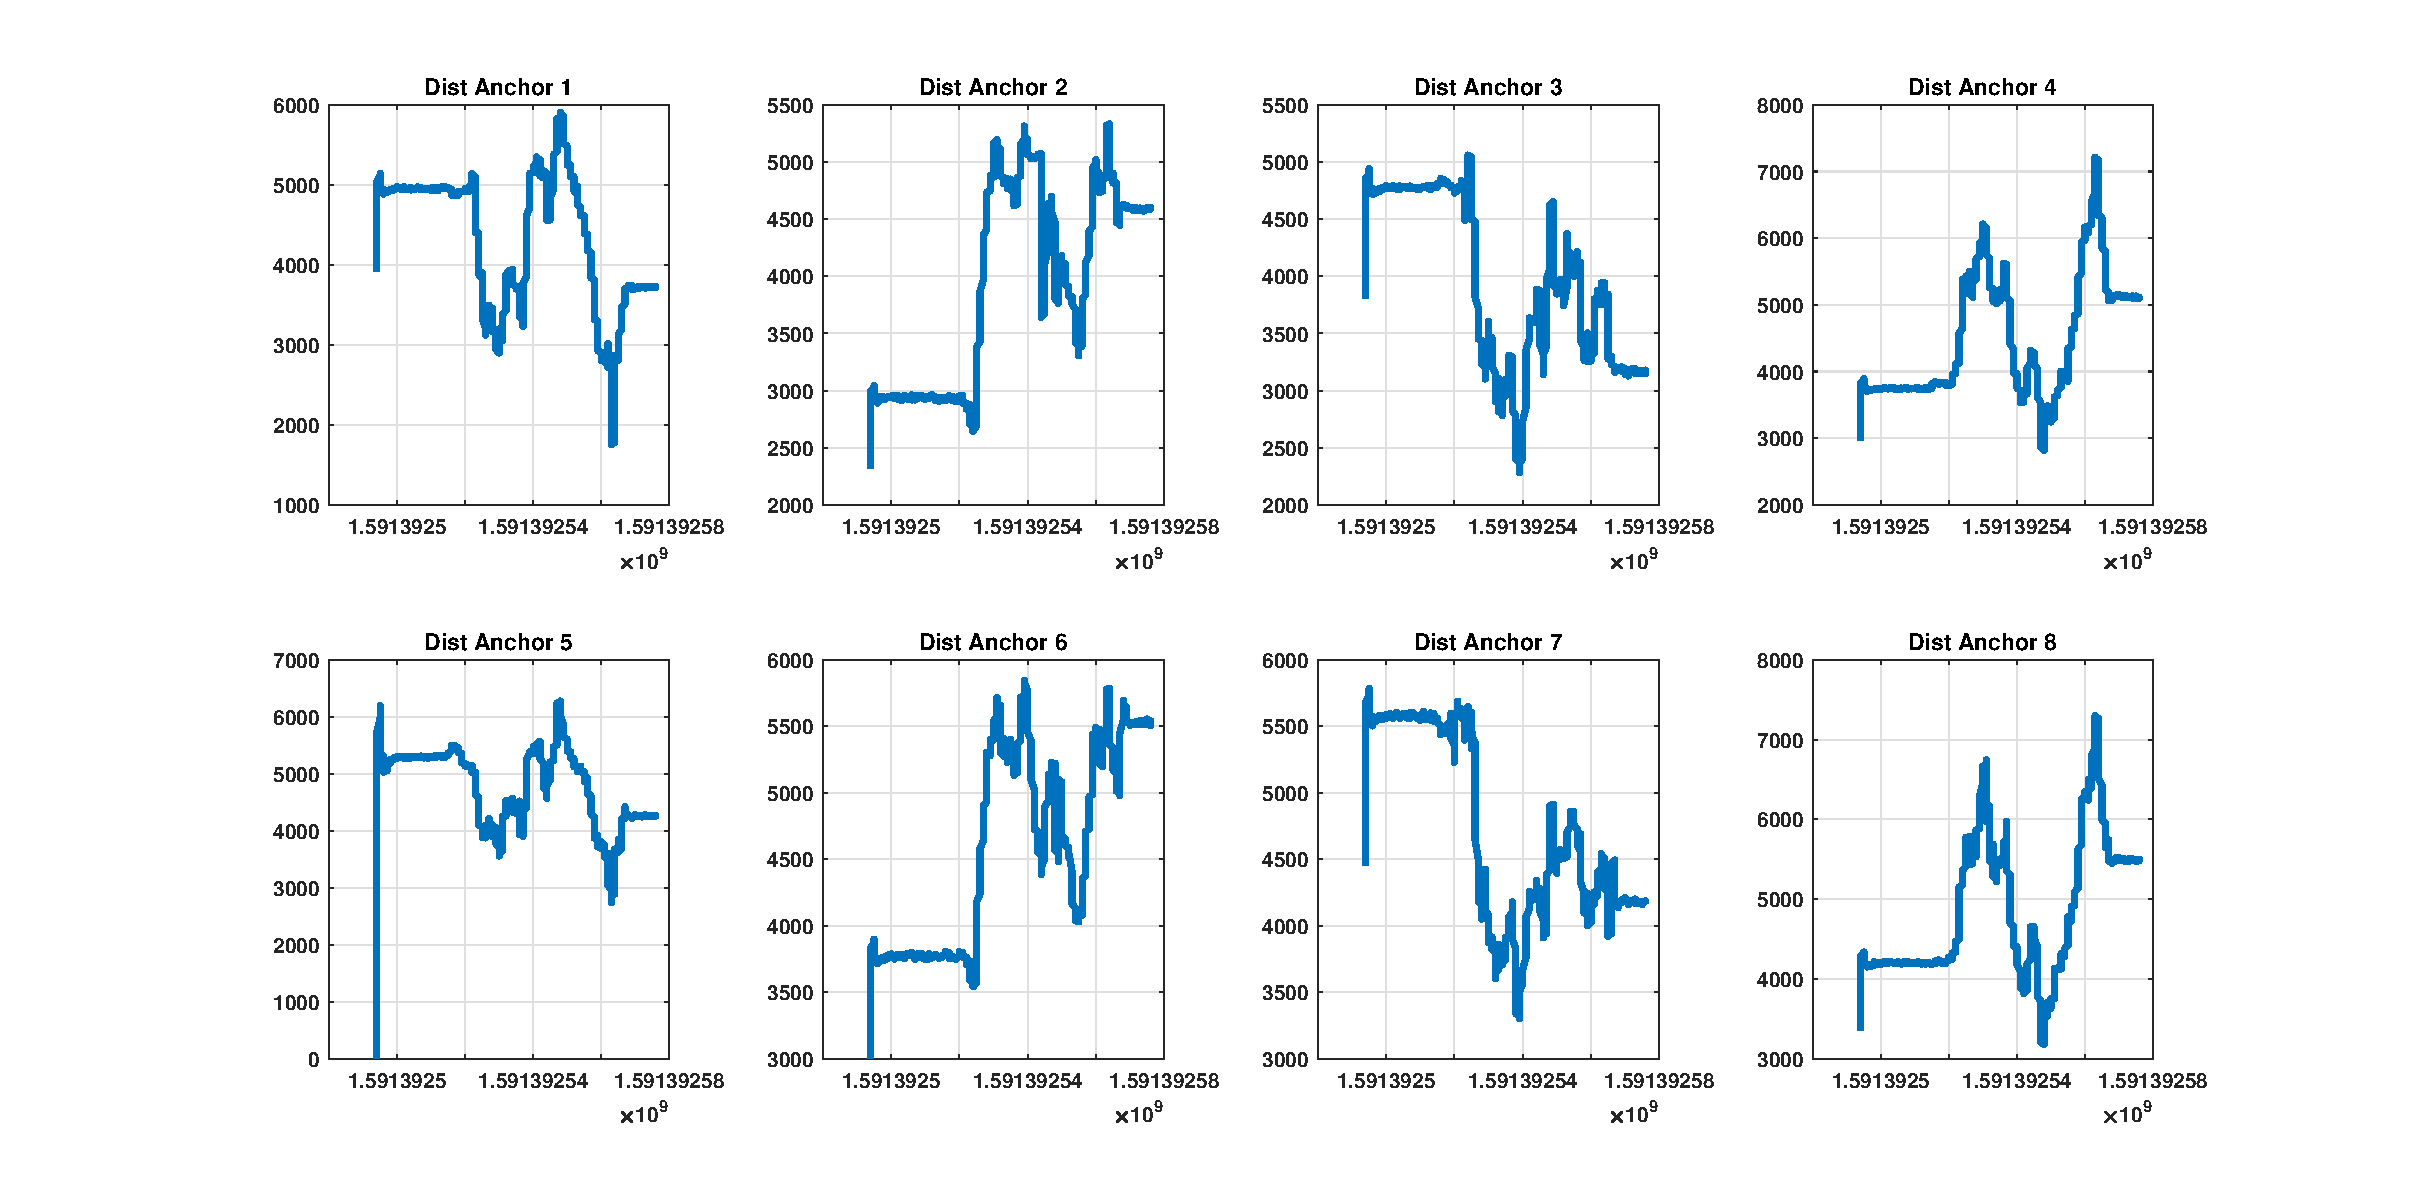
\includegraphics[scale=0.35]{Pics/R05June_Dist.eps}
\caption{The estimated distances to all anchors in the test for evaluating the performance of the velocity estimation algorithm}
\label{Fig_vel_00}
\end{figure}

\begin{figure}[thpb]
\centering
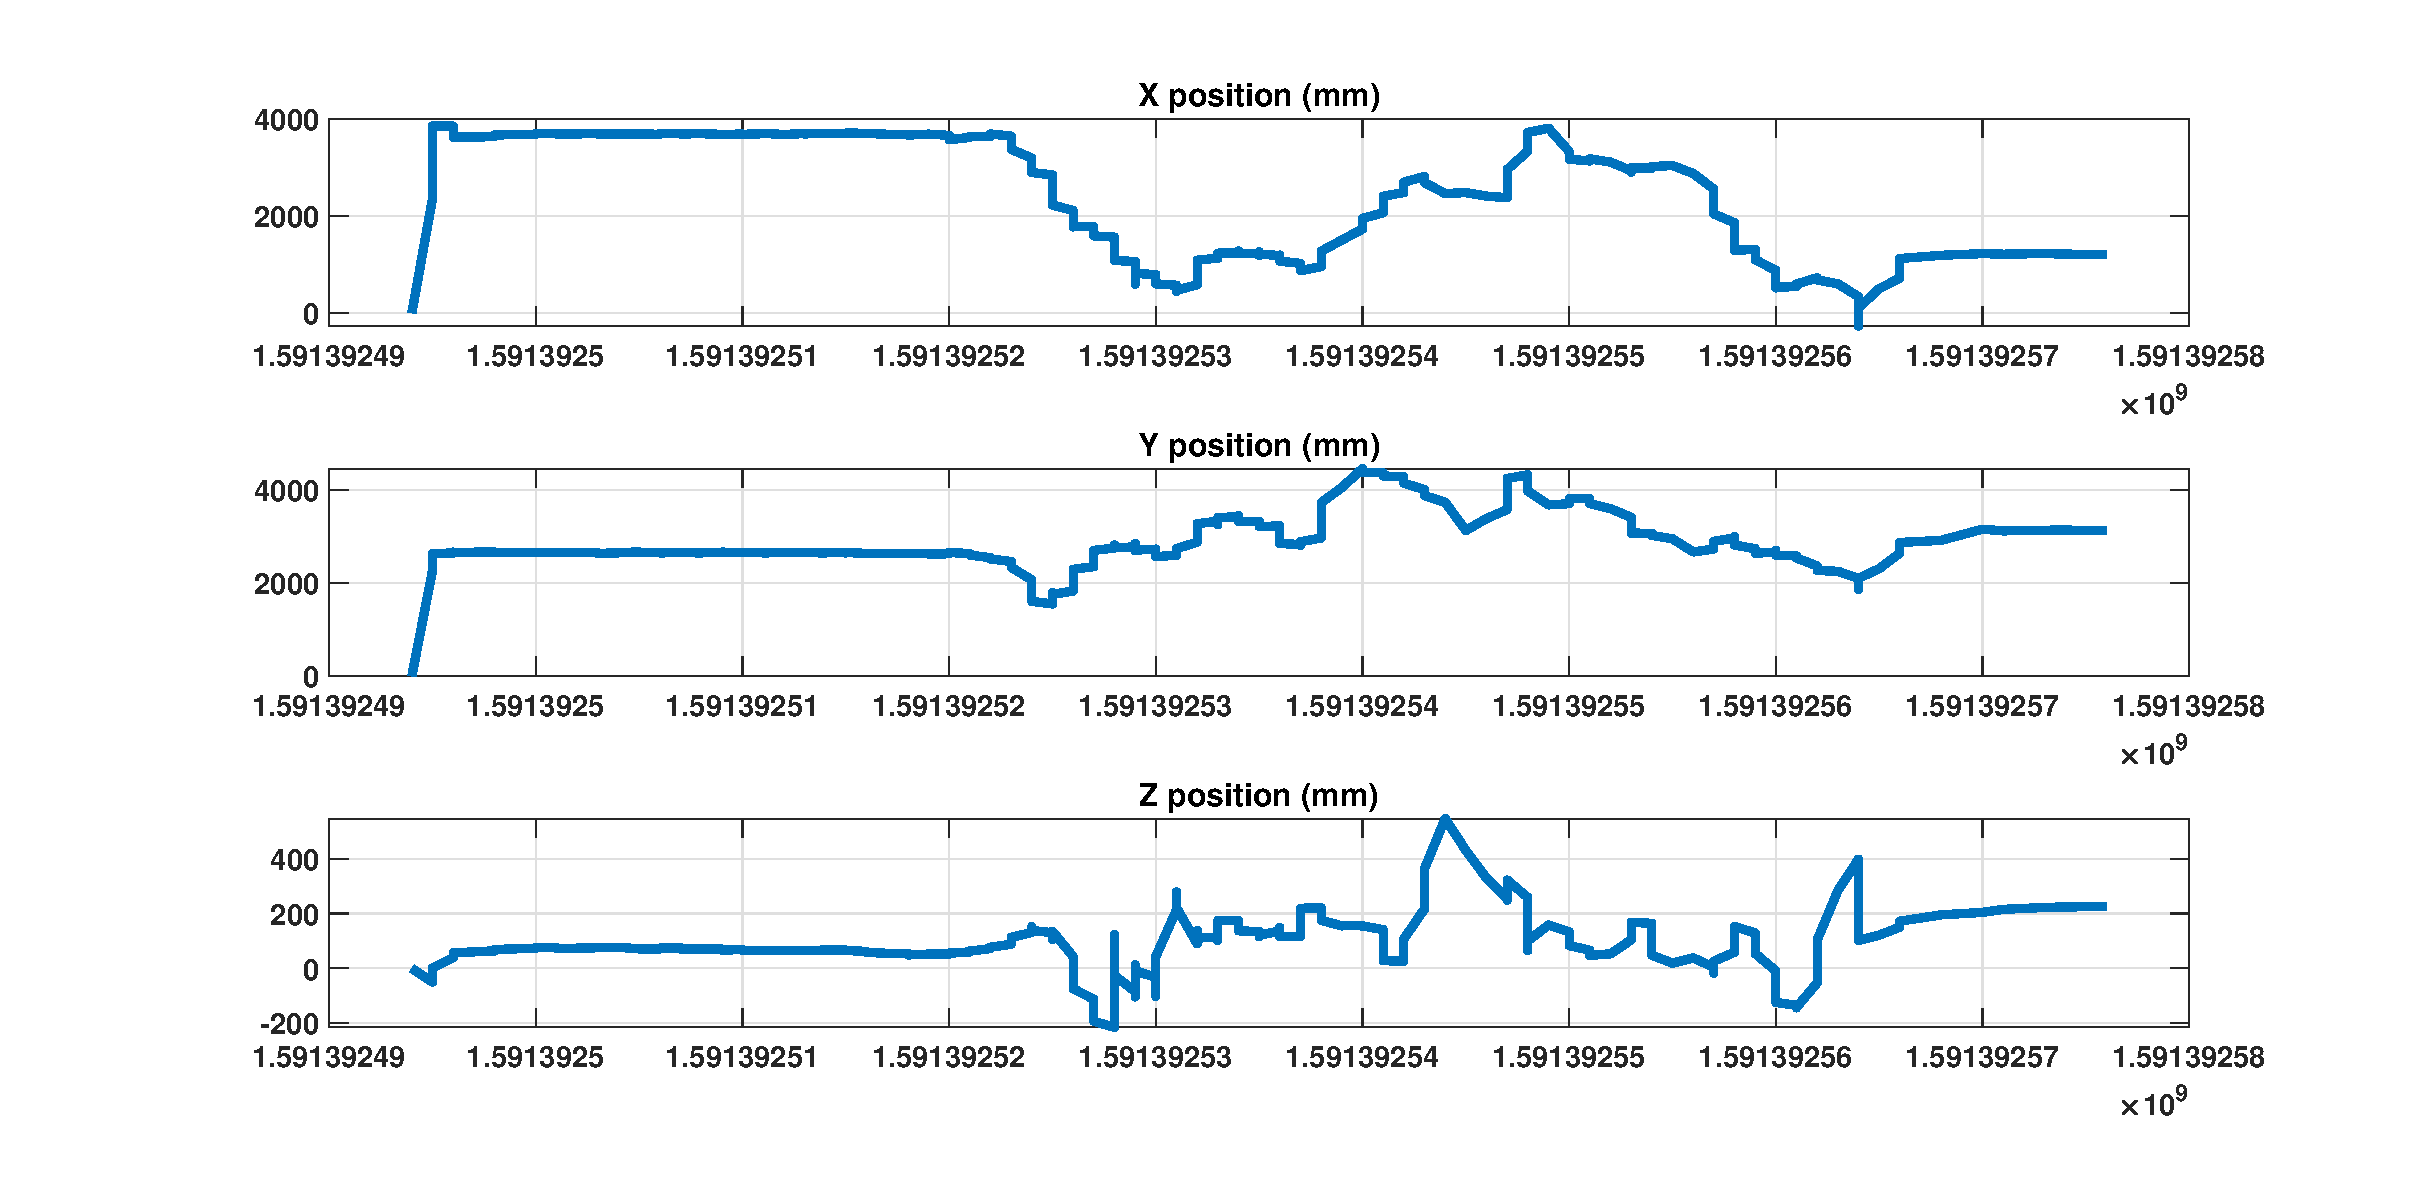
\includegraphics[scale=0.35]{Pics/R05June_Pos.eps}
\caption{The estimated 3D position in the test for evaluating the performance of the velocity estimation algorithm}
\label{Fig_vel_01}
\end{figure}

\begin{figure}[thpb]
\centering
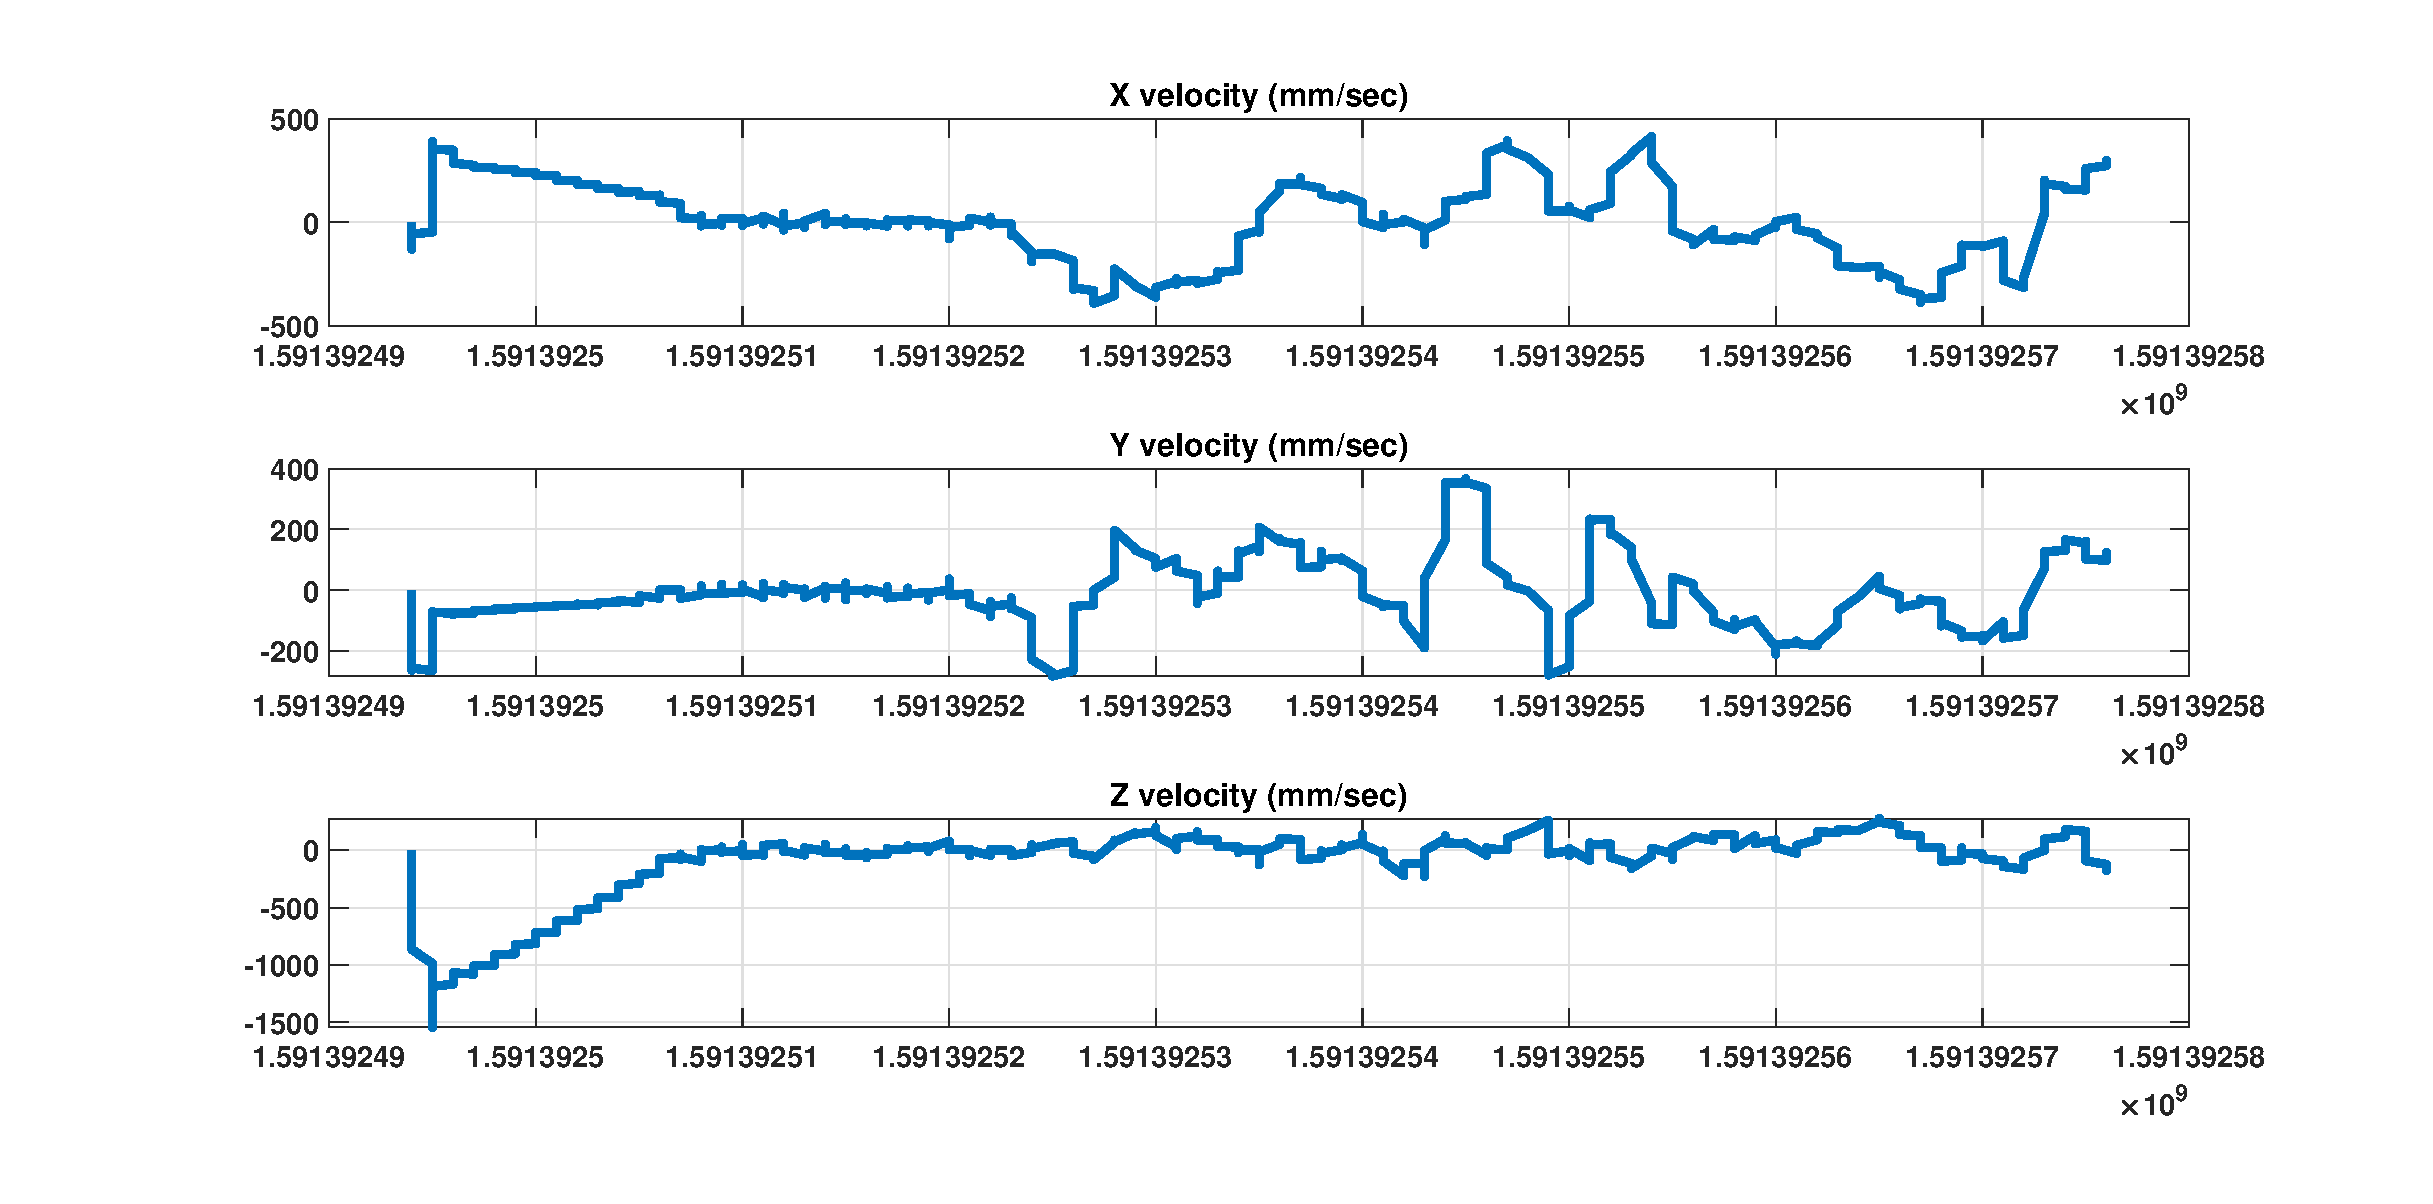
\includegraphics[scale=0.35]{Pics/R05June_Vel.eps}
\caption{The estimated 3D velocity in the test for evaluating the performance of the velocity estimation algorithm}
\label{Fig_vel_02}
\end{figure}

\begin{figure}[thpb]
\centering
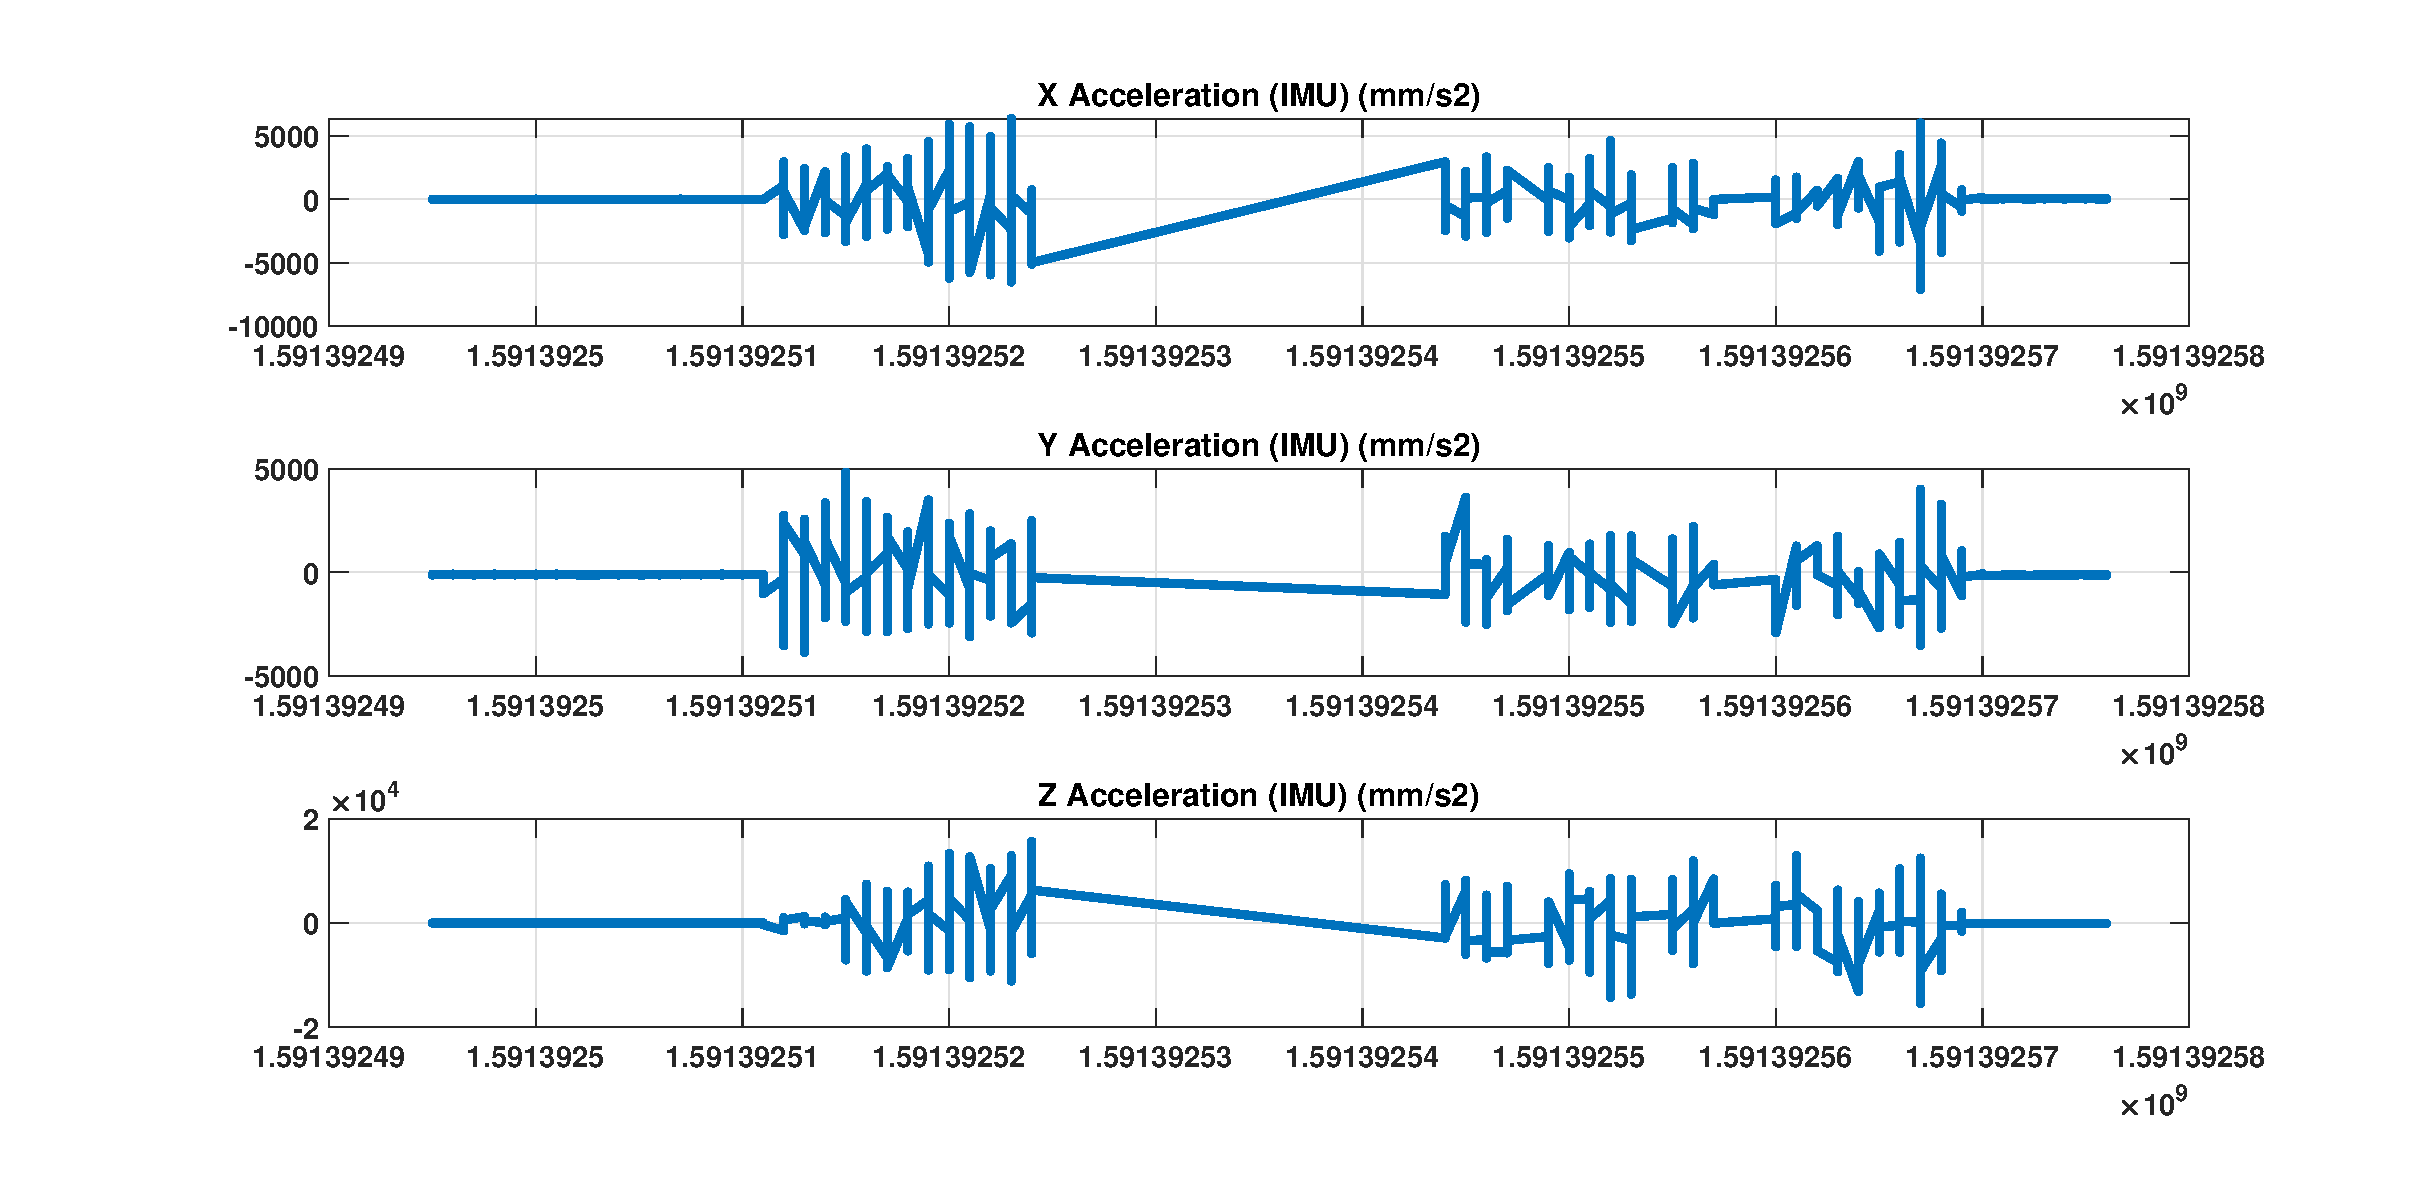
\includegraphics[scale=0.35]{Pics/R05June_Acc.eps}
\caption{The measured acceleration data from PX4 in the test for evaluating the performance of the velocity estimation algorithm}
\label{Fig_vel_03}
\end{figure}

\begin{figure}[thpb]
\centering
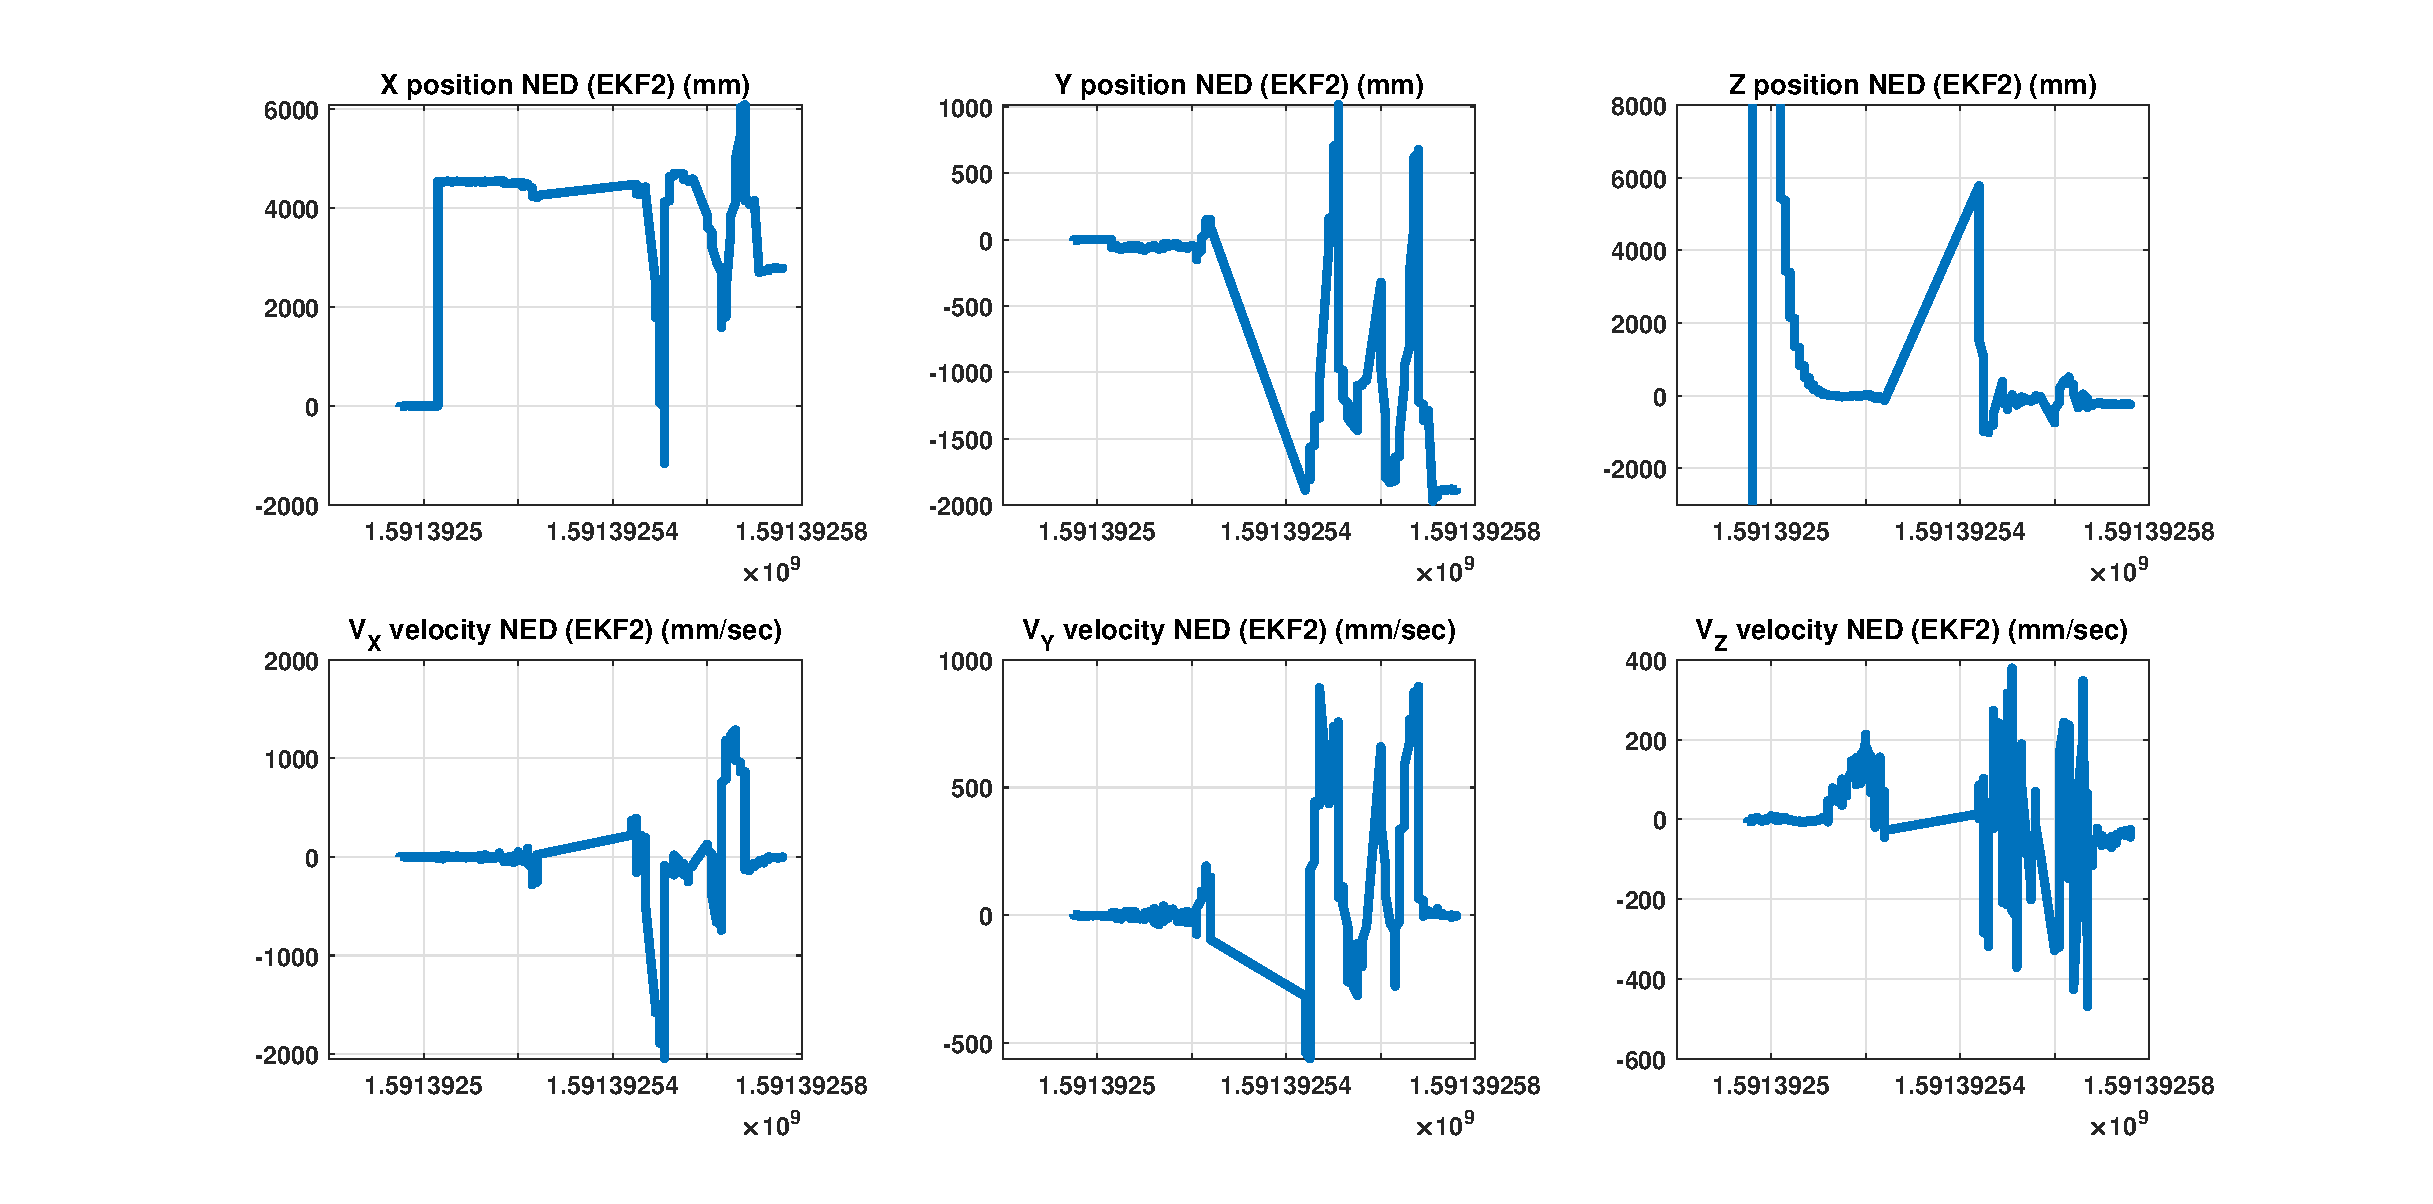
\includegraphics[scale=0.35]{Pics/R05June_EKF2.eps}
\caption{The outputs of EKF2 in the test for evaluating the performance of the velocity estimation algorithm}
\label{Fig_vel_04}
\end{figure}

\begin{figure}[thpb]
\centering
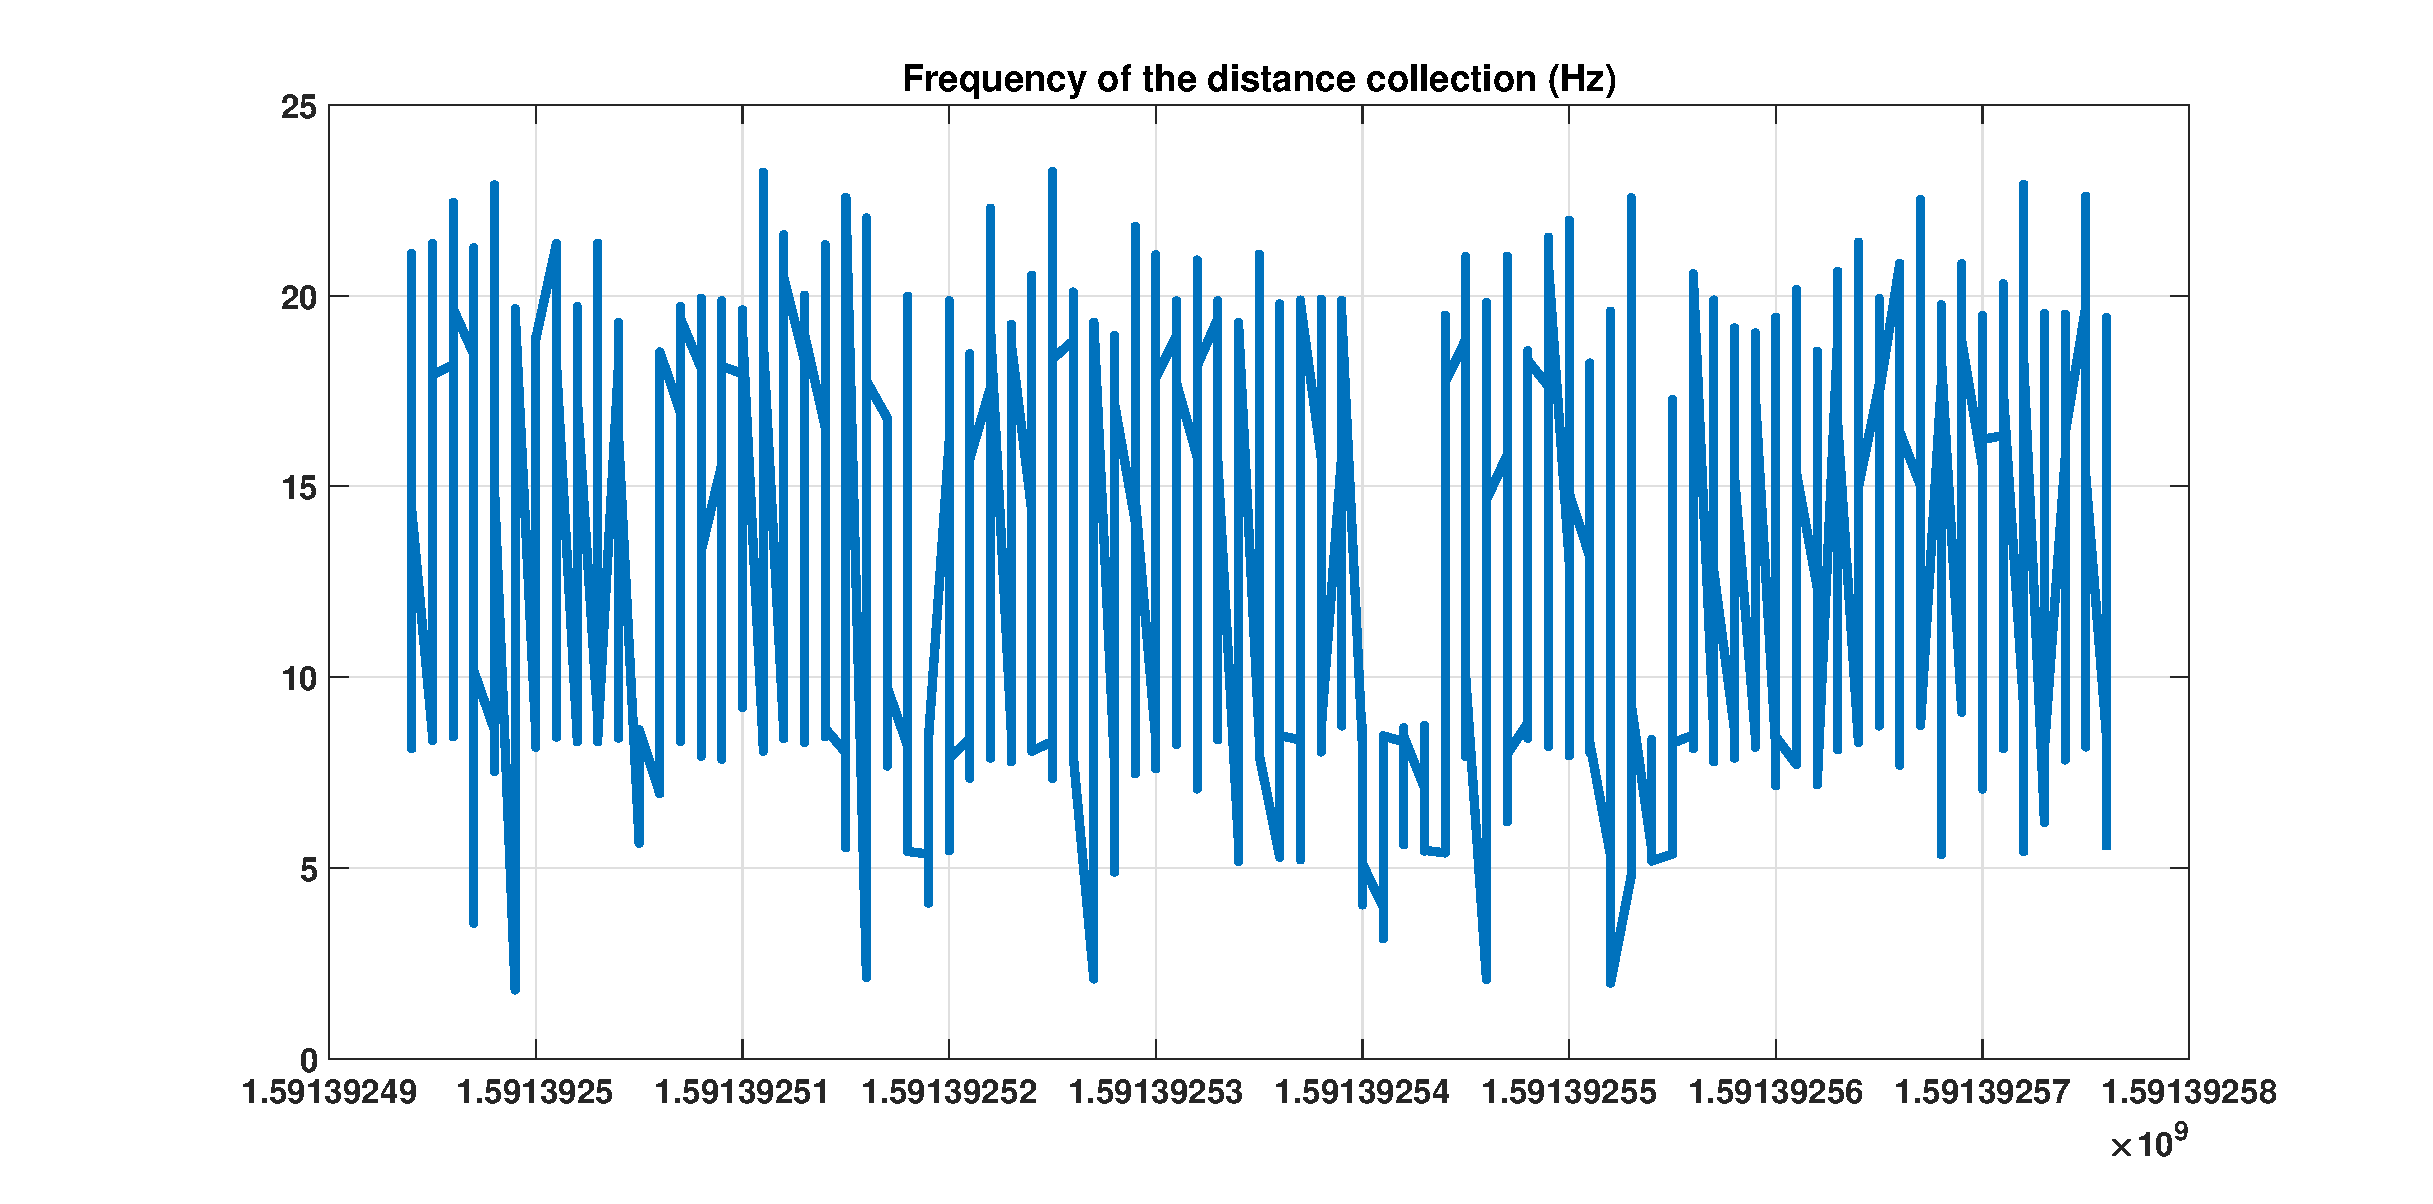
\includegraphics[scale=0.35]{Pics/R05June_Dist_Freq.eps}
\caption{The frequency of distance collections in the test for evaluating the performance of the velocity estimation algorithm}
\label{Fig_vel_05}
\end{figure}

\begin{figure}[thpb]
\centering
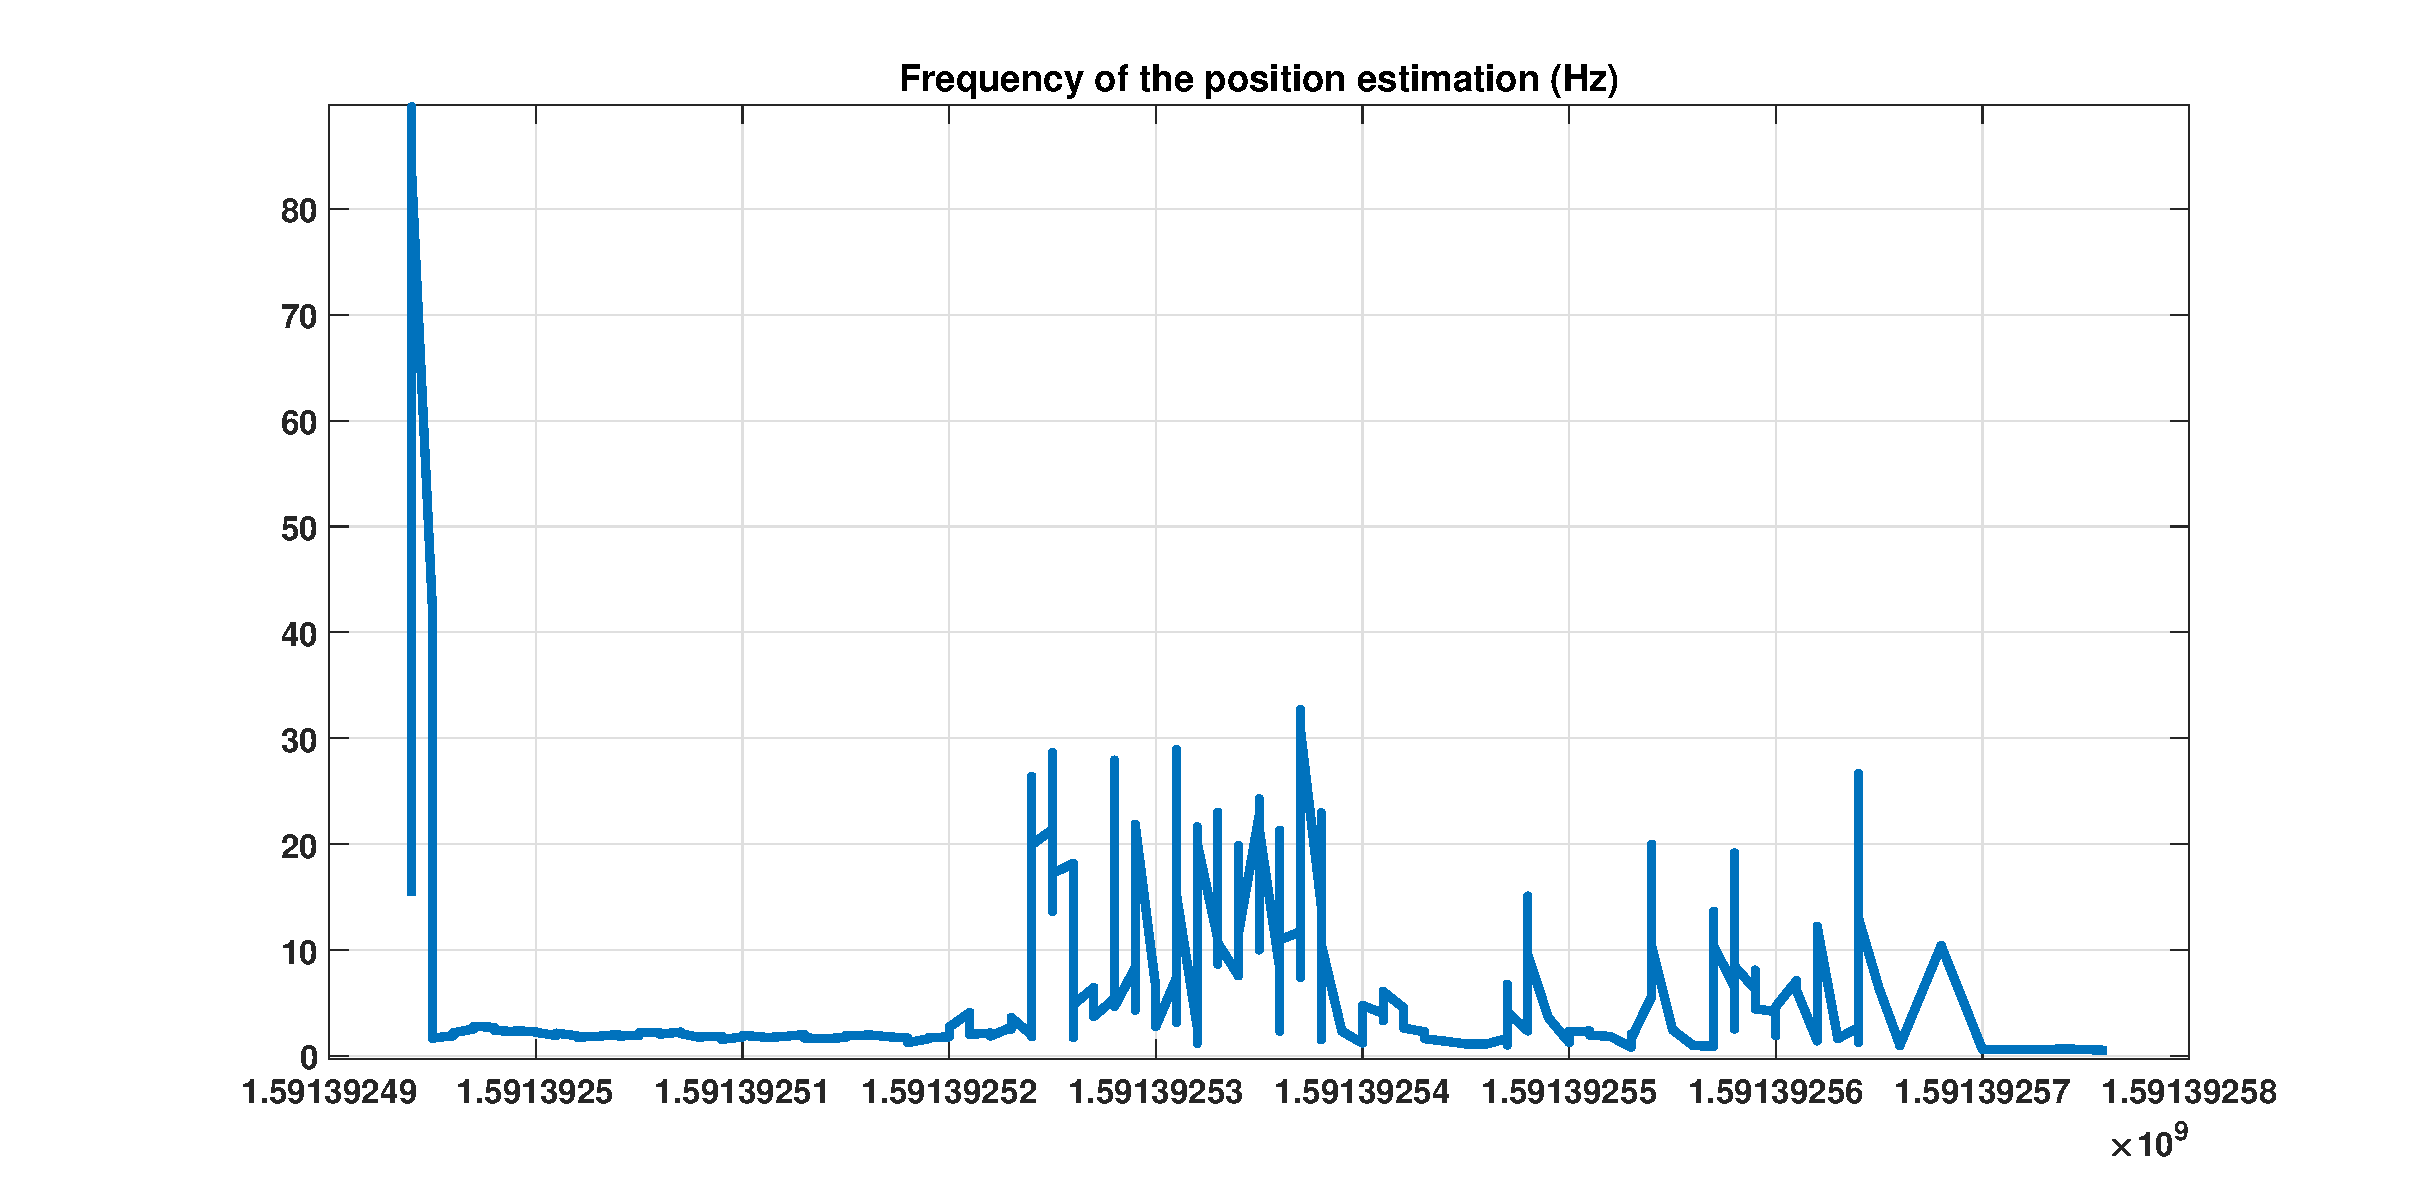
\includegraphics[scale=0.35]{Pics/R05June_Pos_Freq.eps}
\caption{The frequency of the position estimation in the test for evaluating the performance of the velocity estimation algorithm}
\label{Fig_vel_06}
\end{figure}

\begin{figure}[thpb]
\centering
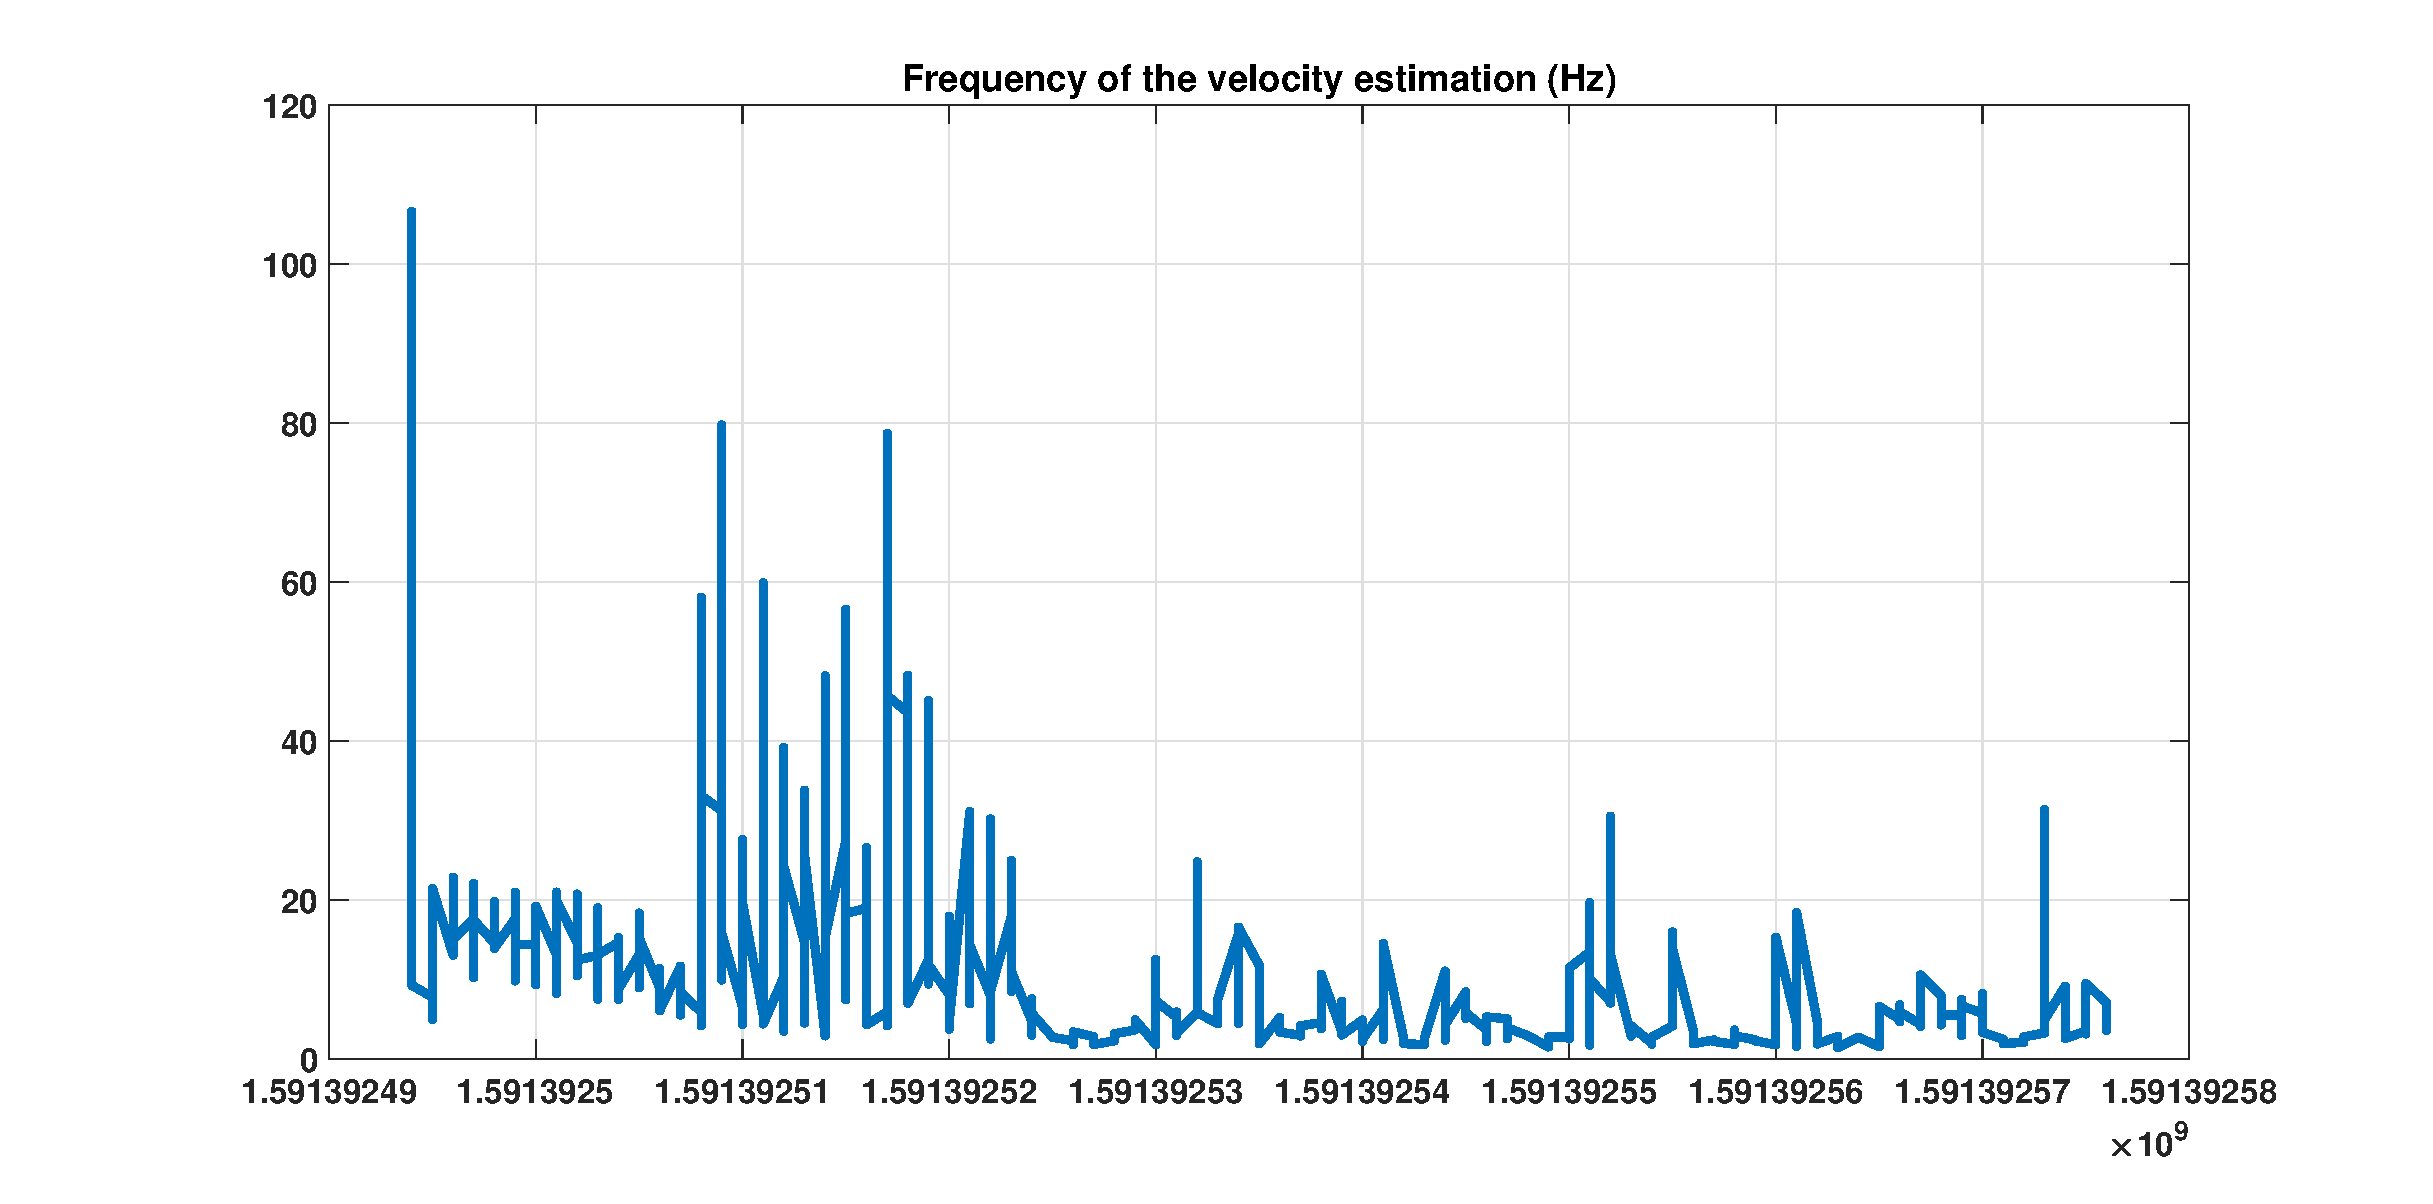
\includegraphics[scale=0.35]{Pics/R05June_Vel_Freq.eps}
\caption{The frequency of the velocity estimation in the test for evaluating the performance of the velocity estimation algorithm}
\label{Fig_vel_07}
\end{figure}



\newpage
\begin{thebibliography}{99}

\bibitem{Slid_Obs1}
Levant, A. Robust exact differentiation via sliding mode technique. \textit{Automatica}. 1998; 34(3): 379-384.

\bibitem{Slid_Obs}
Levant, A. High-order sliding modes, differentiation and output-feedback control. \textit{International Journal of Control}. 2003; 76(9-10): 924-941.

\bibitem{Ali_AMFC01}
Safaei A. and M. N. Mahyuddin, ``Optimal model-free control for a generic MIMO nonlinear system with application to autonomous mobile robots," \textit{International Journal of Adaptive Control and Signal Processing}, Vol. 32, Issue 6, pp. 792-815, 2018.

\bibitem{Ali_AMFC02}
Safaei A. and M. N. Mahyuddin, ``Adaptive model-free control based on an ultra-local model with model-free parameter estimations for a generic SISO system," \textit{IEEE Access}, Vol. 6, pp. 4266-4275, 2018.

\bibitem{Ali_VelEst}
Safaei A., ``Adaptive relative velocity estimation algorithm for autonomous mobile robots using the measurements on acceleration and relative distance," \textit{International Journal of Adaptive Control and Signal Processing}, vol. 34, Issue 3, pp. 372-388, 2020.

\end{thebibliography}


\end{document}
